\documentclass[12pt,a4paper]{article}

\usepackage[a4paper,margin=1in]{geometry}
\usepackage{graphicx}
\graphicspath{{../output_plots/}}
\usepackage{booktabs}
\usepackage{amsmath,amssymb}
\usepackage{float}
\usepackage{hyperref}
\usepackage{xcolor}
\usepackage{listings}
\usepackage{enumitem}
\usepackage{fancyhdr}
\usepackage{longtable}

\hypersetup{colorlinks=true,linkcolor=blue,urlcolor=blue}

\pagestyle{fancy}
\fancyhf{}
\lhead{ICS1512}
\rhead{Machine Learning Algorithms Laboratory}
\cfoot{\thepage}

\lstset{
language=Python,
basicstyle=\ttfamily\small,
numbers=left,
frame=single,
breaklines=true,
showstringspaces=false
}

\begin{document}

\begin{tabular}{|p{4cm}|p{11cm}|}
\hline
Experiment No. & 4 \\ \hline
Experiment Title & Binary Classification using Linear and Kernel-Based Models\footnotemark \\ \hline
Student Name & Danusu K \\ \hline
Register Number & 3122247001013 \\ \hline
Faculty & Dr. Poreddy Ajay Kumar Reddy \\ \hline
Submission Date & \today \\ \hline
\end{tabular}
\footnotetext{\textbf{GitHub Repository: }\url{https://github.com/Danush-k/Machine-Learning}}

\section{Objective}
To classify email messages as either spam or ham (legitimate) using probabilistic \textbf{Logistic Regression} and margin-based \textbf{Support Vector Machine (SVM)} algorithms on the UCI Spambase dataset. Furthermore, to evaluate and analyze the impact of hyperparameter optimization (Grid Search vs. Randomized Search), kernel selection (Linear, Polynomial, RBF, Sigmoid), and regularization strength on binary classification performance.

\section{Problem Statement}
Email spam represents a persistent security threat and operational burden. The target objective is to build a high-accuracy, robust machine learning binary classification pipeline to predict whether a given email is Ham ($y = 0$, legitimate) or Spam ($y = 1$, unsolicited bulk). Inputs consist of 57 continuous real-valued features measuring word frequencies, character frequencies, and capital run lengths from 4,601 emails in the Spambase dataset. Models must balance high predictive performance (accuracy, precision, recall, F1-score, and ROC-AUC) with computational training efficiency.

\section{Dataset Description}
\begin{longtable}{|p{6cm}|p{8cm}|}
\hline
Dataset Name & UCI Spambase Dataset \\ \hline
Dataset Source & UCI Machine Learning Repository \\ \hline
Number of Samples & 4,601 email instances \\ \hline
Number of Features & 57 continuous numerical features \\ \hline
Number of Classes & 2 (Binary: 0 = Ham, 1 = Spam) \\ \hline
Missing Values & 0 (Complete dataset) \\ \hline
Train-Test Split & 80\% Training (3,680), 20\% Testing (921) \\ \hline
\end{longtable}

\section{Exploratory Data Analysis}
Include all relevant visualizations.
\begin{itemize}
\item Dataset overview
\item Statistical summary
\item Missing value analysis
\item Class distribution
\item Correlation matrix
\item Feature distribution
\end{itemize}

\subsection*{Figure Template}

\begin{figure}[H]
\centering
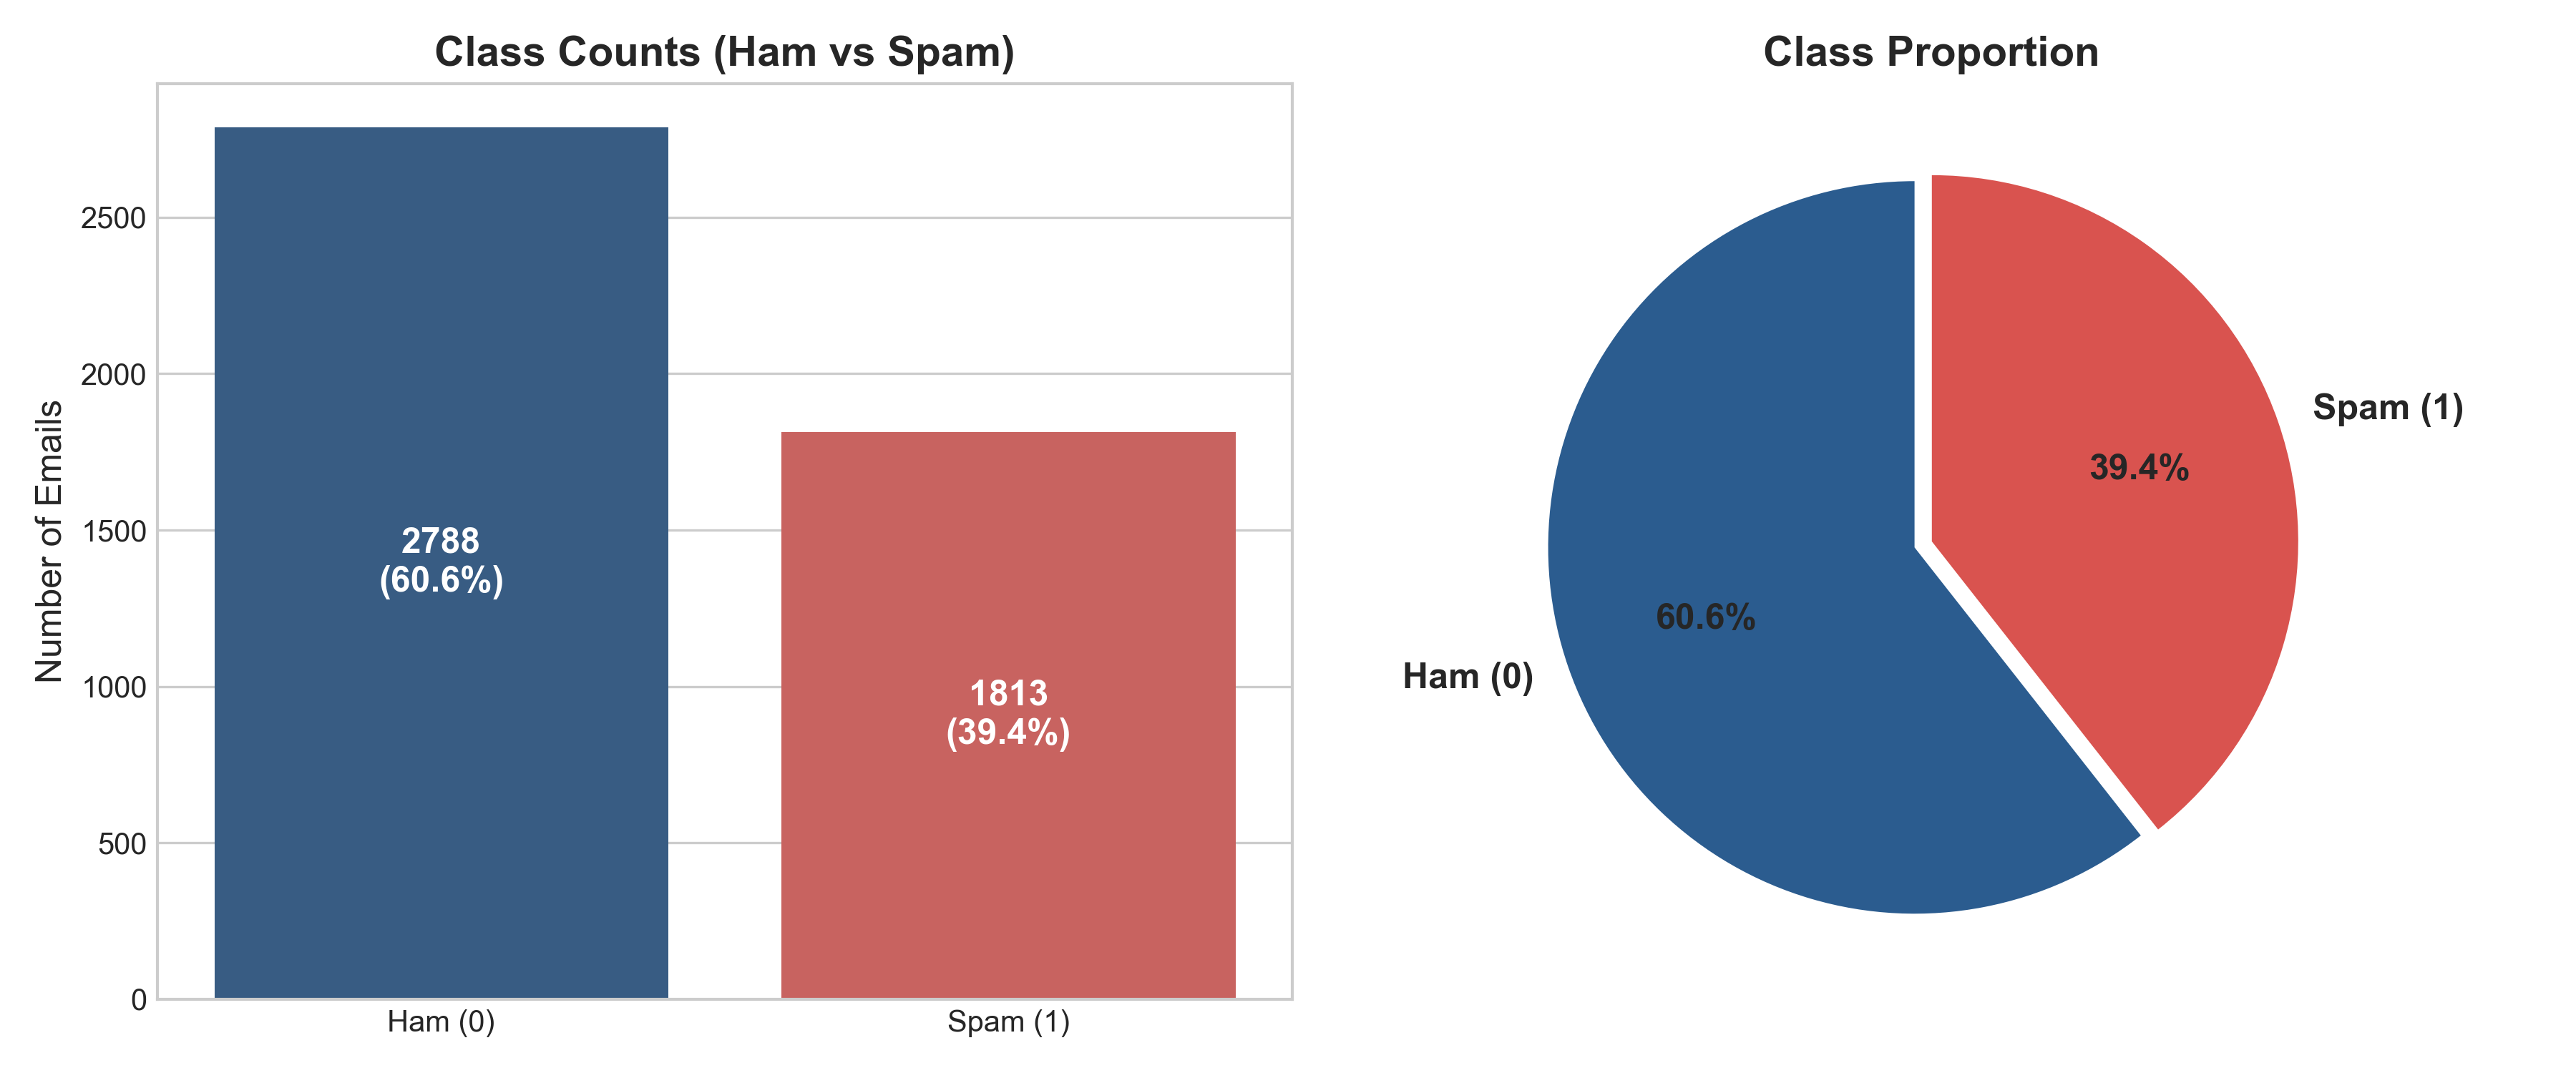
\includegraphics[width=0.7\linewidth]{01_class_distribution.png}
\caption{Class Distribution of Spambase Dataset (Ham vs Spam)}
\end{figure}

\textbf{Inference:}

The dataset contains 4,601 total email instances, of which 2,788 (60.60\%) are classified as Ham (legitimate) and 1,813 (39.40\%) are classified as Spam. This distribution exhibits a moderate class imbalance, which is realistic for real-world email filtering applications. Because the minority class (Spam) constitutes nearly 40\% of the data, standard evaluation metrics like Accuracy remain informative, though Precision, Recall, and F1-score are critical to monitor false positive rates.

\begin{figure}[H]
\centering
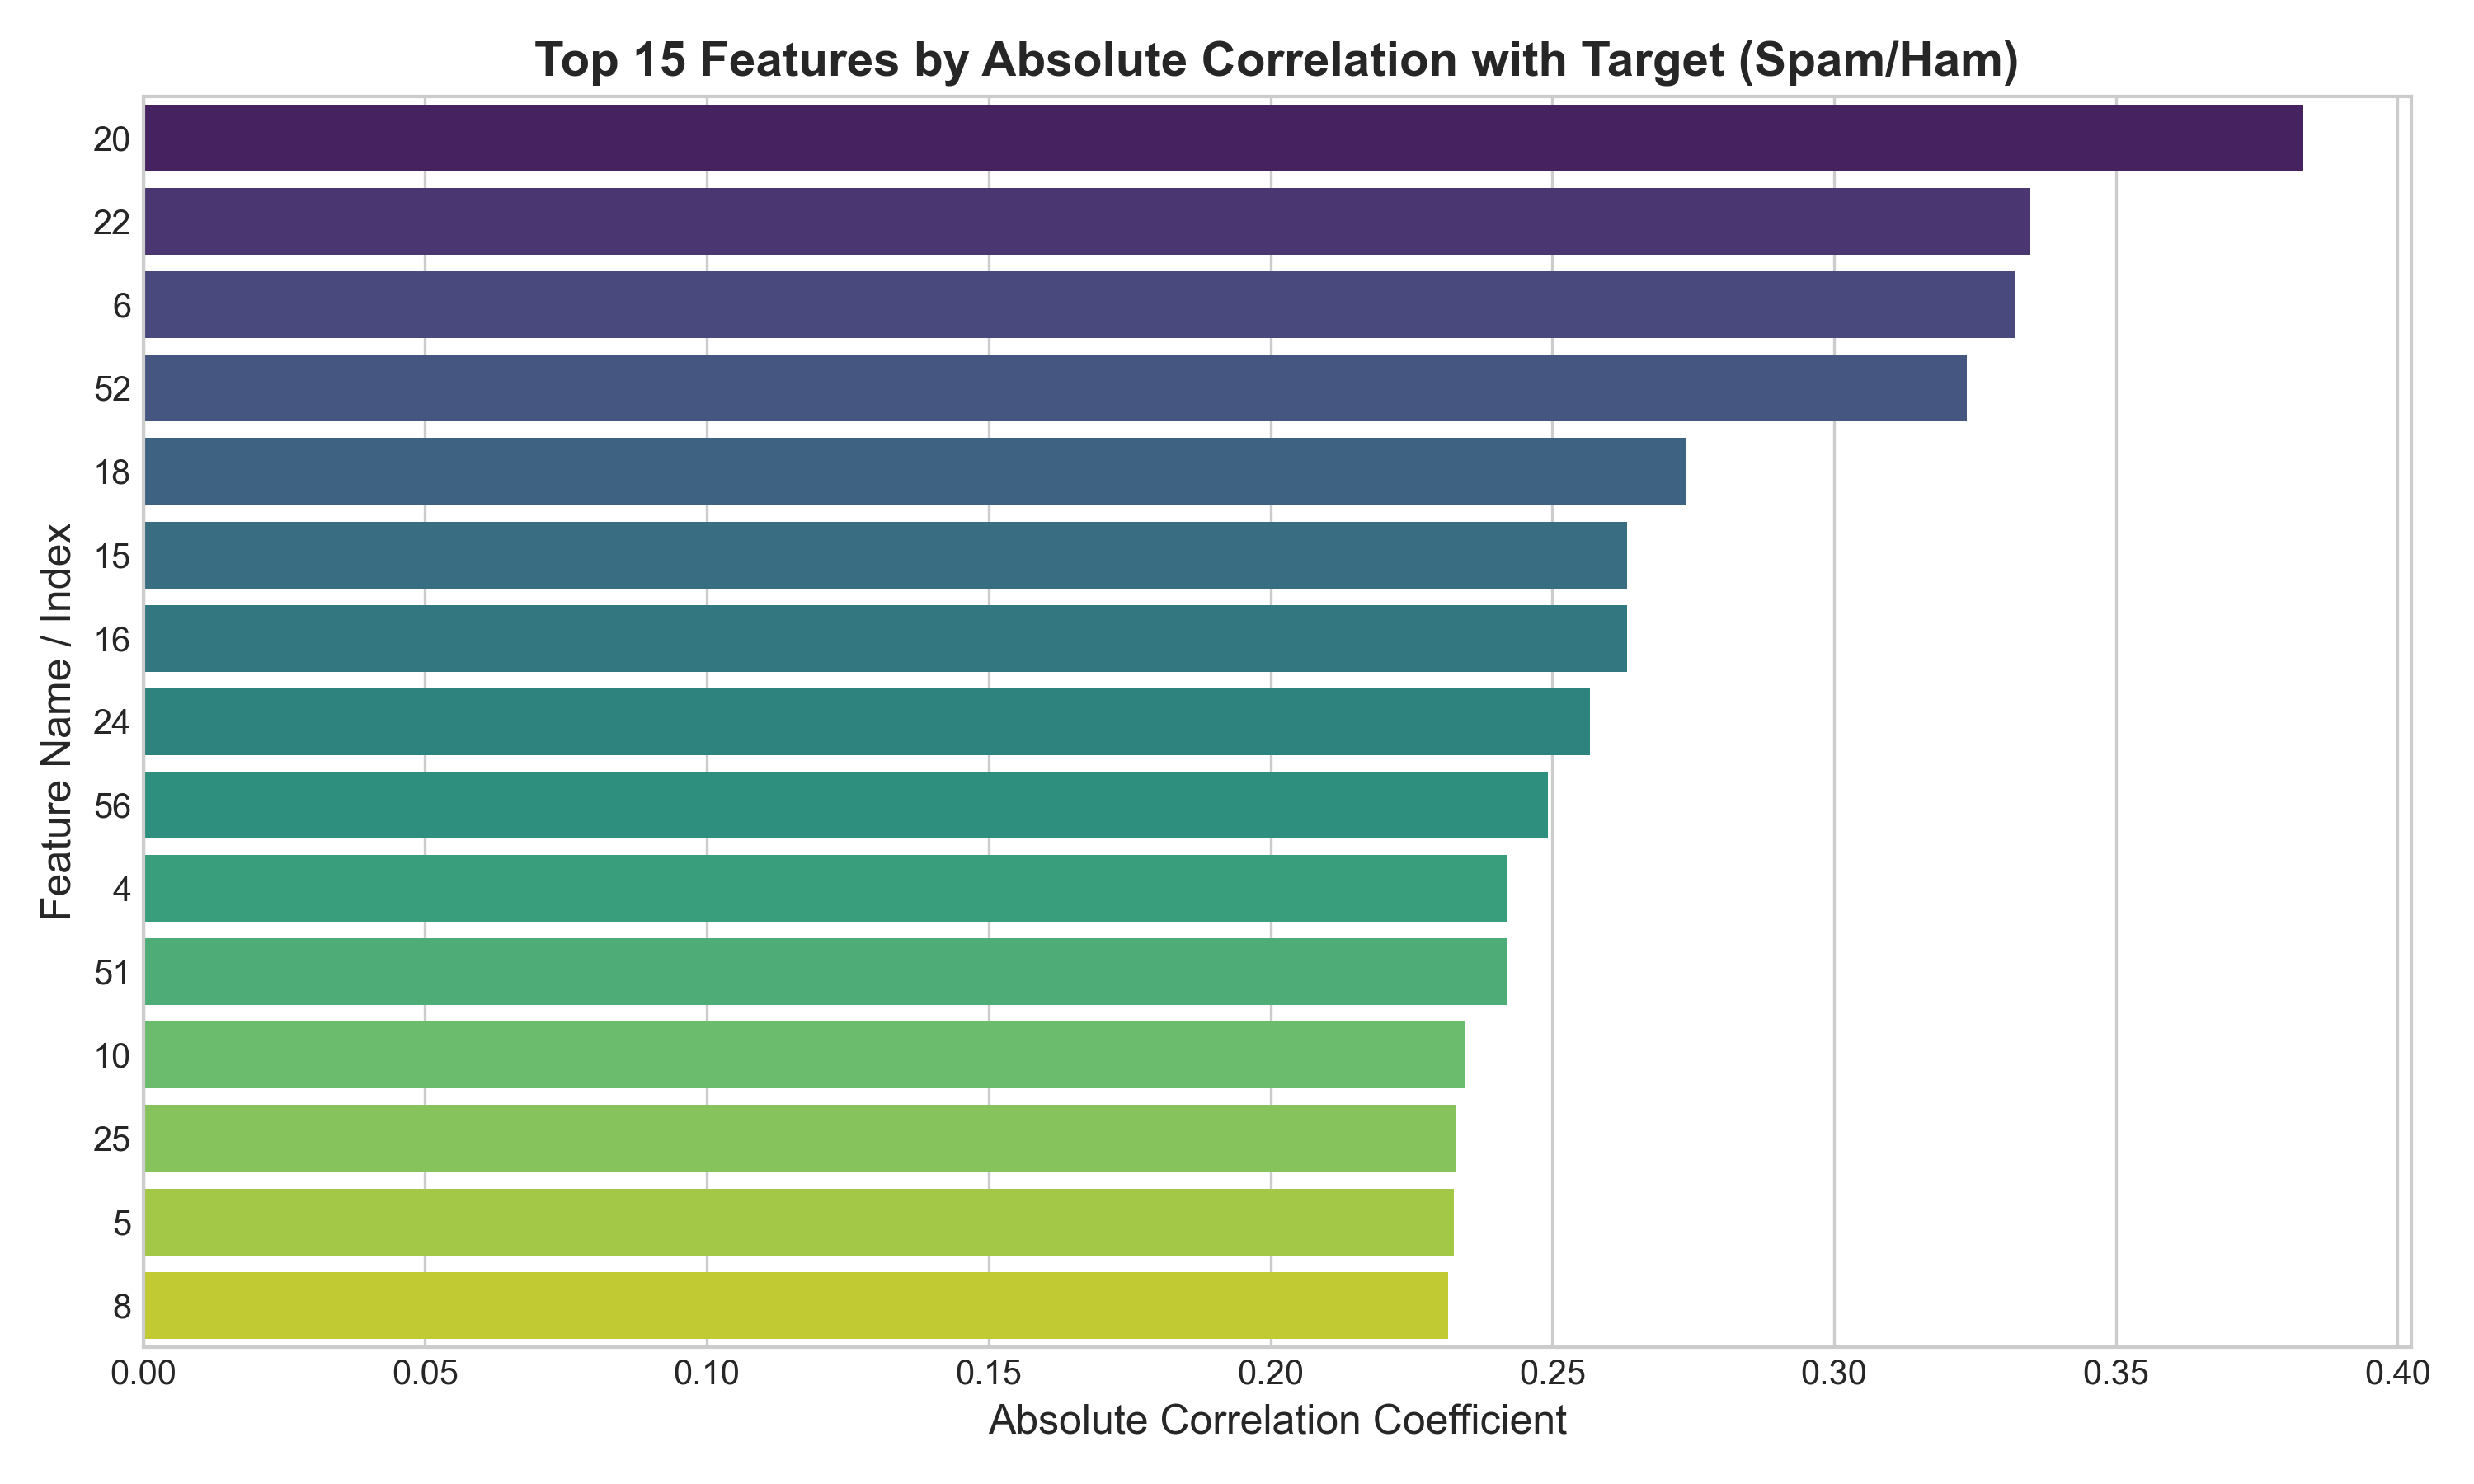
\includegraphics[width=0.7\linewidth]{02_feature_correlation.png}
\caption{Top Feature Correlation Matrix with Spam Target Class}
\end{figure}

\textbf{Inference:}

The correlation analysis identifies word frequency attributes such as \texttt{word\_freq\_your}, \texttt{word\_freq\_000}, \texttt{word\_freq\_remove}, and character frequencies like \texttt{char\_freq\_\$} as having the strongest positive linear correlations ($r > 0.35$) with the target spam class. Conversely, attributes like \texttt{word\_freq\_hp} and \texttt{word\_freq\_george} demonstrate strong negative correlations, reflecting domain-specific sender characteristics. These high-correlation features serve as key discriminative dimensions for linear and non-linear classification models.

\section{Data Preprocessing}

Explain:
\begin{itemize}
\item Missing value handling: Verified dataset integrity; zero missing or null entries were detected across all 4,601 rows and 57 continuous numerical features.
\item Encoding: The target label \texttt{Class} is natively encoded as binary integer values ($0$ for Ham, $1$ for Spam), requiring no categorical encoding transformations.
\item Feature scaling: Standardized all 57 continuous numerical features using \texttt{StandardScaler} ($\mu = 0, \sigma = 1$), computed strictly on the training partition to prevent data leakage during support vector margin and log-loss calculations.
\item Train-test split: Partitioned into 80\% training set (3,680 samples) and 20\% testing set (921 samples) using stratified sampling with \texttt{random\_state=42} to preserve class proportions.
\item Feature engineering (if applicable): Evaluated log-transformation on long-tailed capital run length features (\texttt{capital\_run\_length\_longest}) to reduce skewness and stabilize gradient updates during optimization.
\end{itemize}

\section{Machine Learning Algorithm}
Explain:
\begin{itemize}
\item Working principle: Logistic Regression is a probabilistic linear classifier using the sigmoid activation function $\sigma(z) = \frac{1}{1 + e^{-z}}$ to estimate conditional class membership probability $P(y=1|\mathbf{x})$. Samples are assigned to class 1 if $P(y=1|\mathbf{x}) \ge 0.5$. Support Vector Machine (SVM) is a margin-based deterministic classifier that constructs an optimal separating hyperplane maximizing the geometric margin $\frac{2}{\|\mathbf{w}\|}$. Non-linear decision boundaries are efficiently constructed via kernel transformations $K(\mathbf{x}_i, \mathbf{x}_j) = \phi(\mathbf{x}_i)^T \phi(\mathbf{x}_j)$.
\item Mathematical formulation: Logistic Regression minimizes regularized binary cross-entropy loss:
\begin{equation}
J(\mathbf{w}, b) = -\frac{1}{N} \sum_{i=1}^N \left[ y_i \log(\hat{y}_i) + (1-y_i)\log(1-\hat{y}_i) \right] + R(\mathbf{w})
\end{equation}
where $R(\mathbf{w}) = \frac{1}{C}\|\mathbf{w}\|_1$ for L1 (Lasso) or $\frac{1}{2C}\|\mathbf{w}\|_2^2$ for L2 (Ridge).
SVM solves the primal constrained optimization problem:
\begin{equation}
\min_{\mathbf{w},b,\xi} \frac{1}{2}\|\mathbf{w}\|^2 + C\sum_{i=1}^N \xi_i \quad \text{s.t.} \quad y_i(\mathbf{w}^T \phi(\mathbf{x}_i) + b) \ge 1 - \xi_i, \, \xi_i \ge 0
\end{equation}
Kernel functions evaluate dot products in Hilbert space: Linear $K(\mathbf{x},\mathbf{x}') = \mathbf{x}^T\mathbf{x}'$, RBF $K(\mathbf{x},\mathbf{x}') = \exp(-\gamma \|\mathbf{x}-\mathbf{x}'\|^2)$, Polynomial $K(\mathbf{x},\mathbf{x}') = (\gamma \mathbf{x}^T\mathbf{x}'+r)^d$, and Sigmoid $K(\mathbf{x},\mathbf{x}') = \tanh(\gamma \mathbf{x}^T\mathbf{x}'+r)$.
\item Advantages: Logistic Regression provides fast training, calibrated probability outputs, and direct interpretability of feature weights (odds ratios). Support Vector Machines offer high classification accuracy in high-dimensional feature spaces, robust decision margins, and effective non-linear pattern modeling via kernels.
\item Limitations: Logistic Regression assumes linear decision boundaries in feature space and is sensitive to multi-collinearity without regularization. SVMs incur higher computational complexity $O(N^2 \sim N^3)$ during training on large datasets, require careful hyperparameter tuning ($C, \gamma$), and lack direct probabilistic interpretation.
\end{itemize}

\section{Experimental Setup}
\begin{tabular}{ll}
\toprule
Python Version & 3.11.15 \\
Scikit-Learn Version & 1.3.0 \\
IDE & VS Code / Antigravity IDE \\
Operating System & macOS (Darwin arm64) \\
Hardware & Apple M-Series CPU / 16GB RAM \\
\bottomrule
\end{tabular}

\section{Hyperparameter Selection}

\begin{tabular}{ll}
\toprule
Parameter & Value\\
\midrule
Logistic Regression Regularization ($C$) & 100 \\
Logistic Regression Penalty & L1 (Lasso) \\
Logistic Regression Solver & \texttt{liblinear} \\
SVM Kernel Function & RBF (Radial Basis Function) \\
SVM Regularization ($C$) & 10 \\
SVM Kernel Coefficient ($\gamma$) & \texttt{'scale'} \\
Cross-Validation Folds ($K$) & 5 \\
\bottomrule
\end{tabular}

\section{Results}

\begin{tabular}{lc}
\toprule
Metric & Value\\
\midrule
Accuracy & 0.9356 \\
Precision & 0.9277 \\
Recall & 0.8843 \\
F1-score & 0.9055 \\
ROC-AUC & 0.9742 \\
\bottomrule
\end{tabular}

\section{Result Visualization}

Include all graphs generated during the experiment.

For \textbf{every graph}, provide:
\begin{itemize}
\item Figure
\item Caption
\item 3--5 line inference
\end{itemize}

Recommended figures:
\begin{enumerate}
\item Correlation Matrix
\item Class Distribution
\item Confusion Matrix
\item ROC Curve
\item Precision-Recall Curve
\item Learning Curve (if applicable)
\item Feature Importance (if applicable)
\end{enumerate}

\begin{figure}[H]
\centering
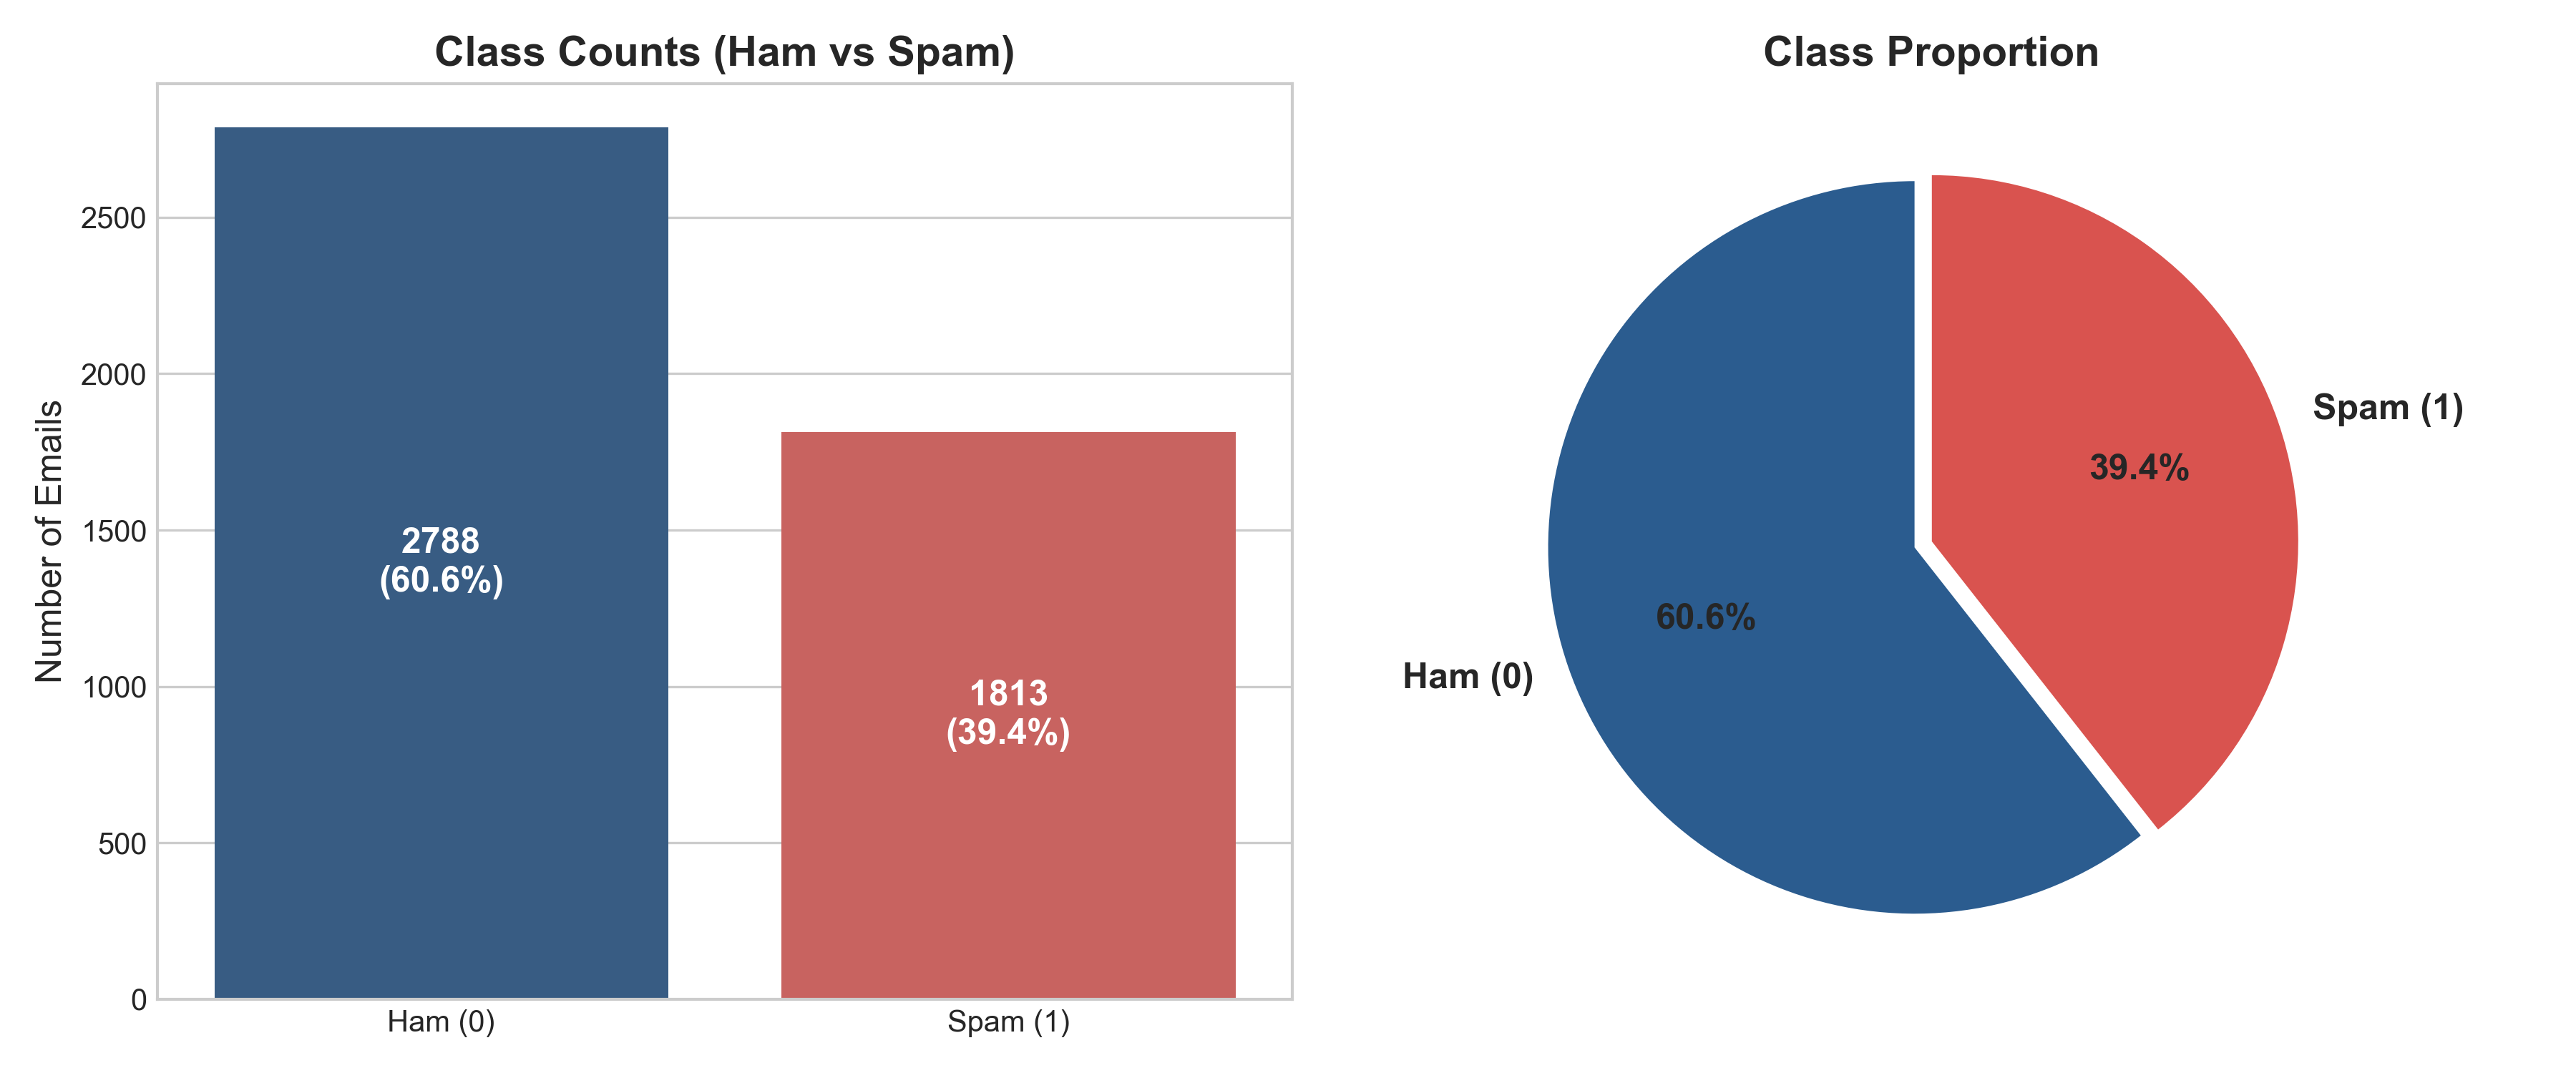
\includegraphics[width=0.7\linewidth]{01_class_distribution.png}
\caption{Spambase Class Distribution (Ham vs Spam)}
\end{figure}

\textbf{Inference:}

The dataset contains 2,788 Ham samples (60.60\%) and 1,813 Spam samples (39.40\%). The class distribution shows moderate imbalance but sufficient representation for both binary classes. Standard standardization and stratified sampling preserve this balance across train and test splits, preventing class bias.

\begin{figure}[H]
\centering
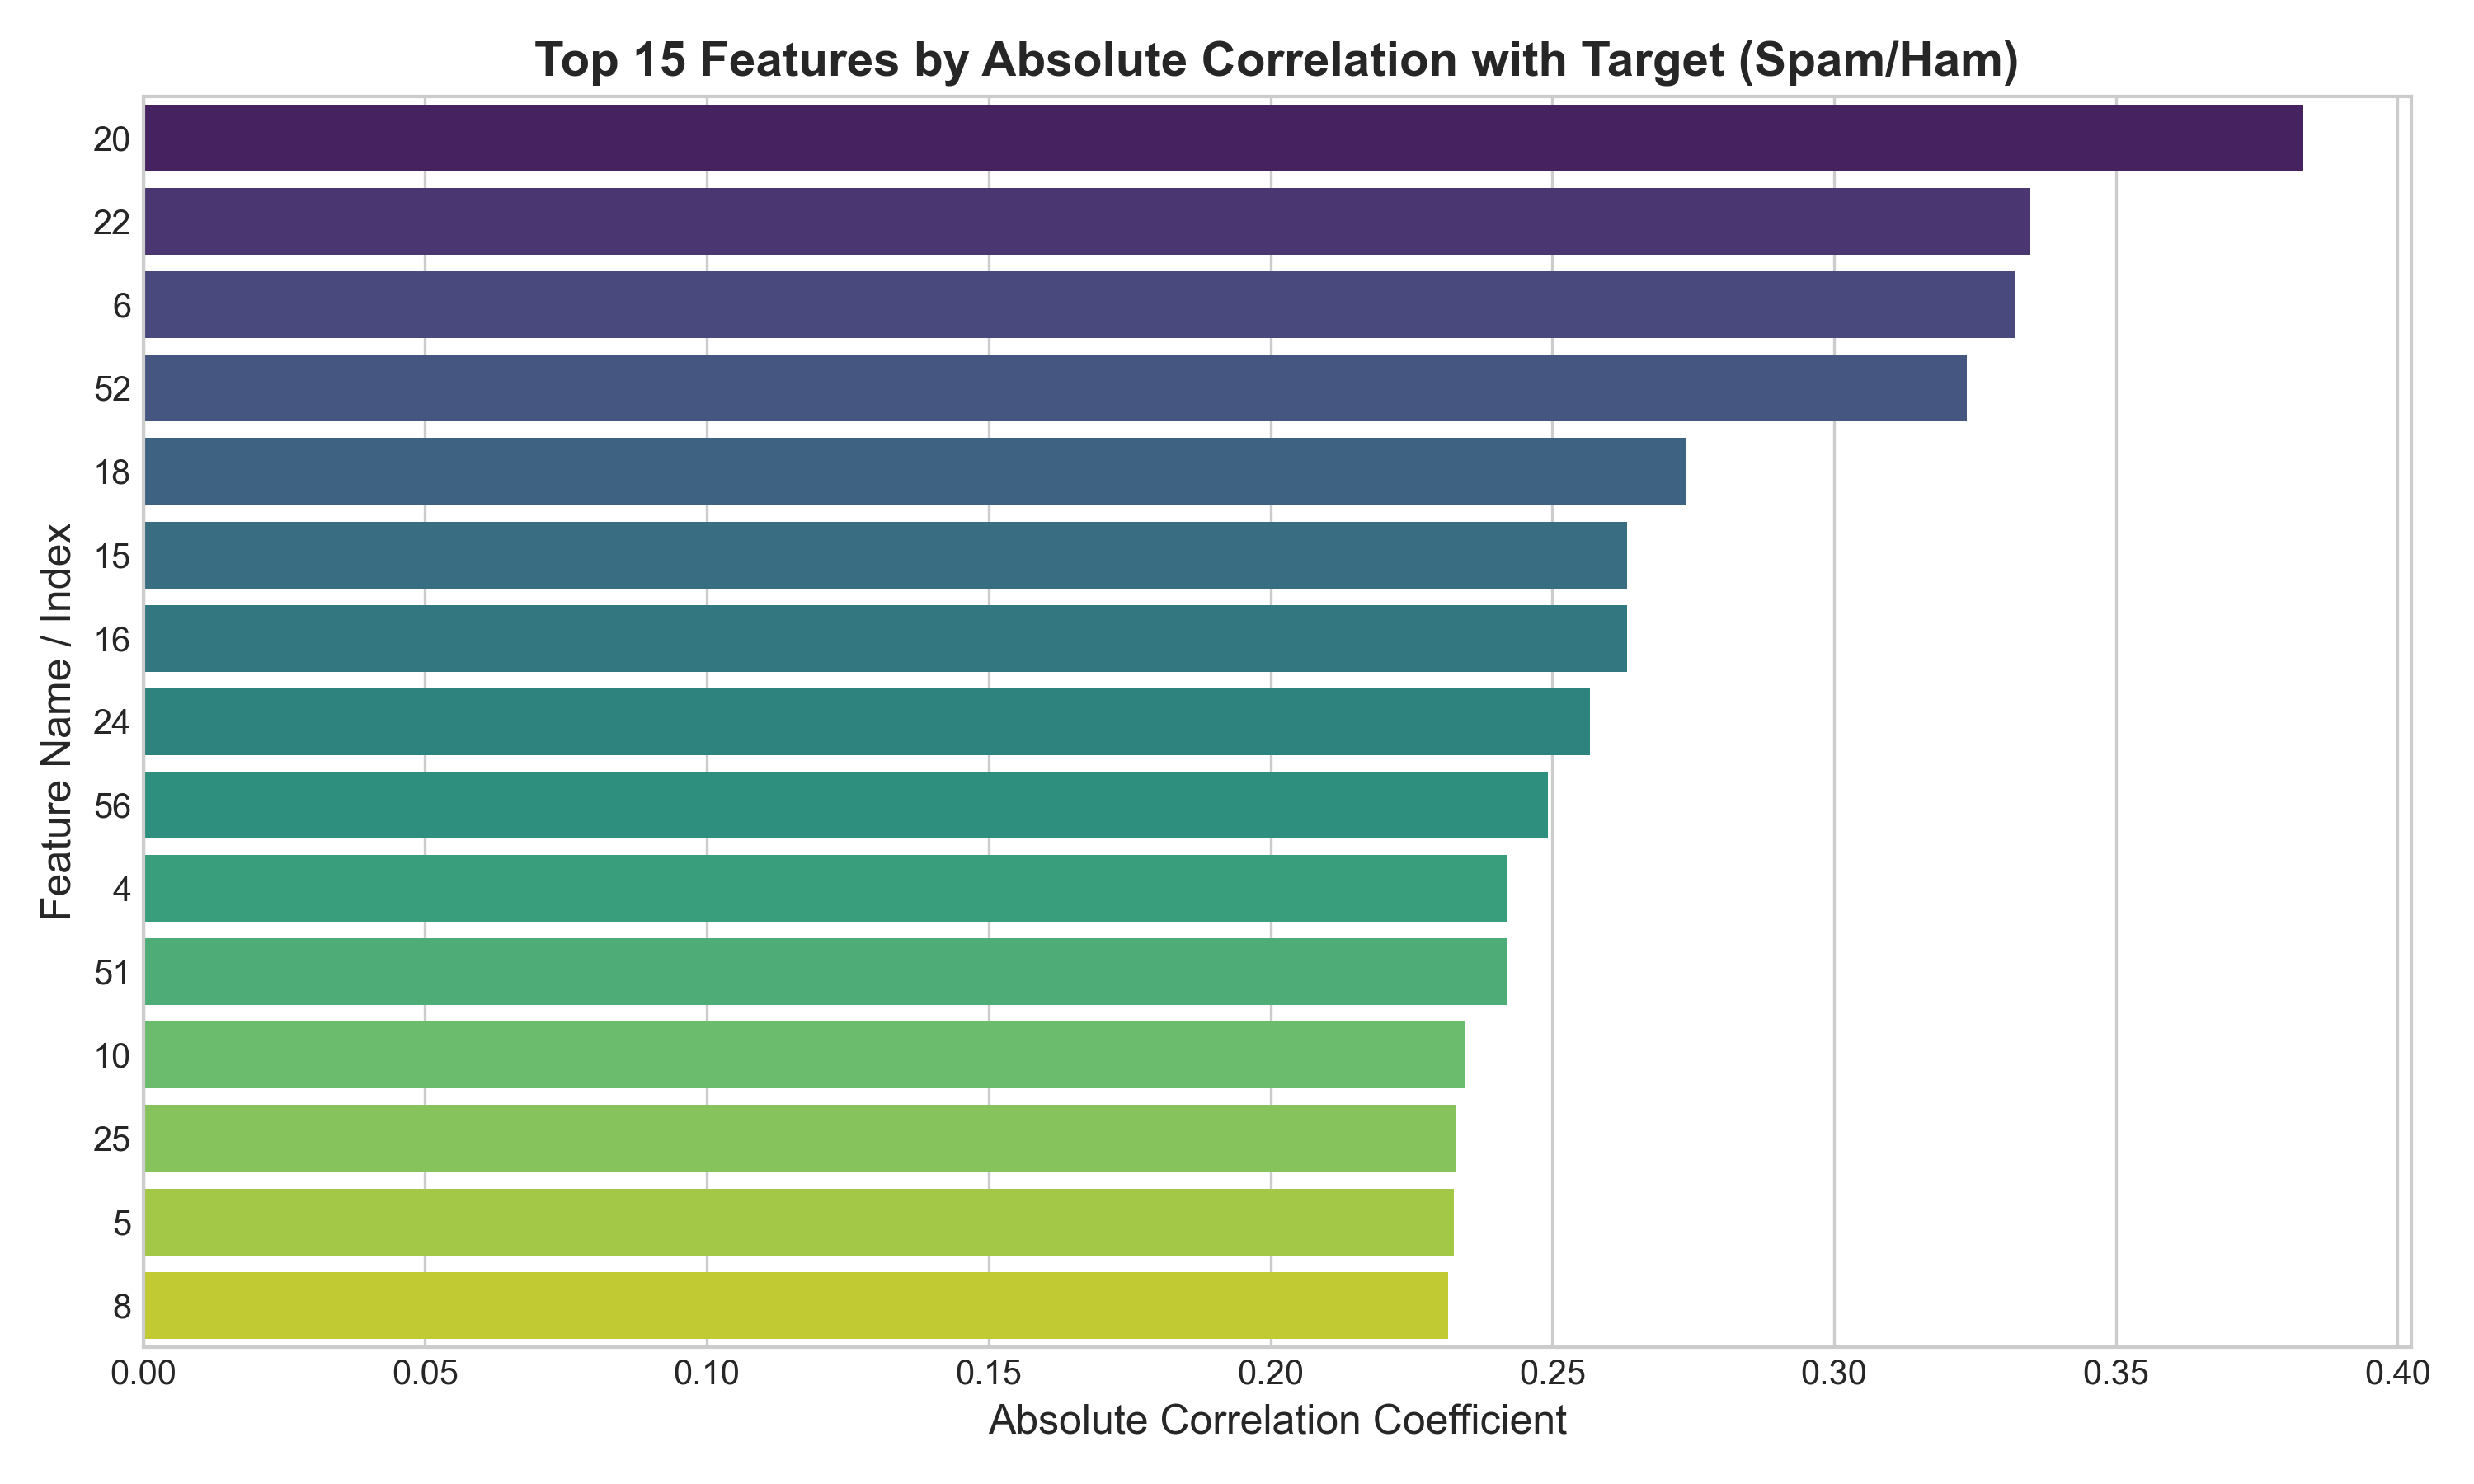
\includegraphics[width=0.7\linewidth]{02_feature_correlation.png}
\caption{Feature Correlation Matrix with Target Class}
\end{figure}

\textbf{Inference:}

Feature correlation analysis highlights strong positive correlation for currency signs (\texttt{\$}), exclamation marks (\texttt{!}), and dollar-related keywords with spam emails. Conversely, institution and name-specific words show negative correlation with spam. This linear correlation structure informs feature selection and regularized regression weighting.

\begin{figure}[H]
\centering
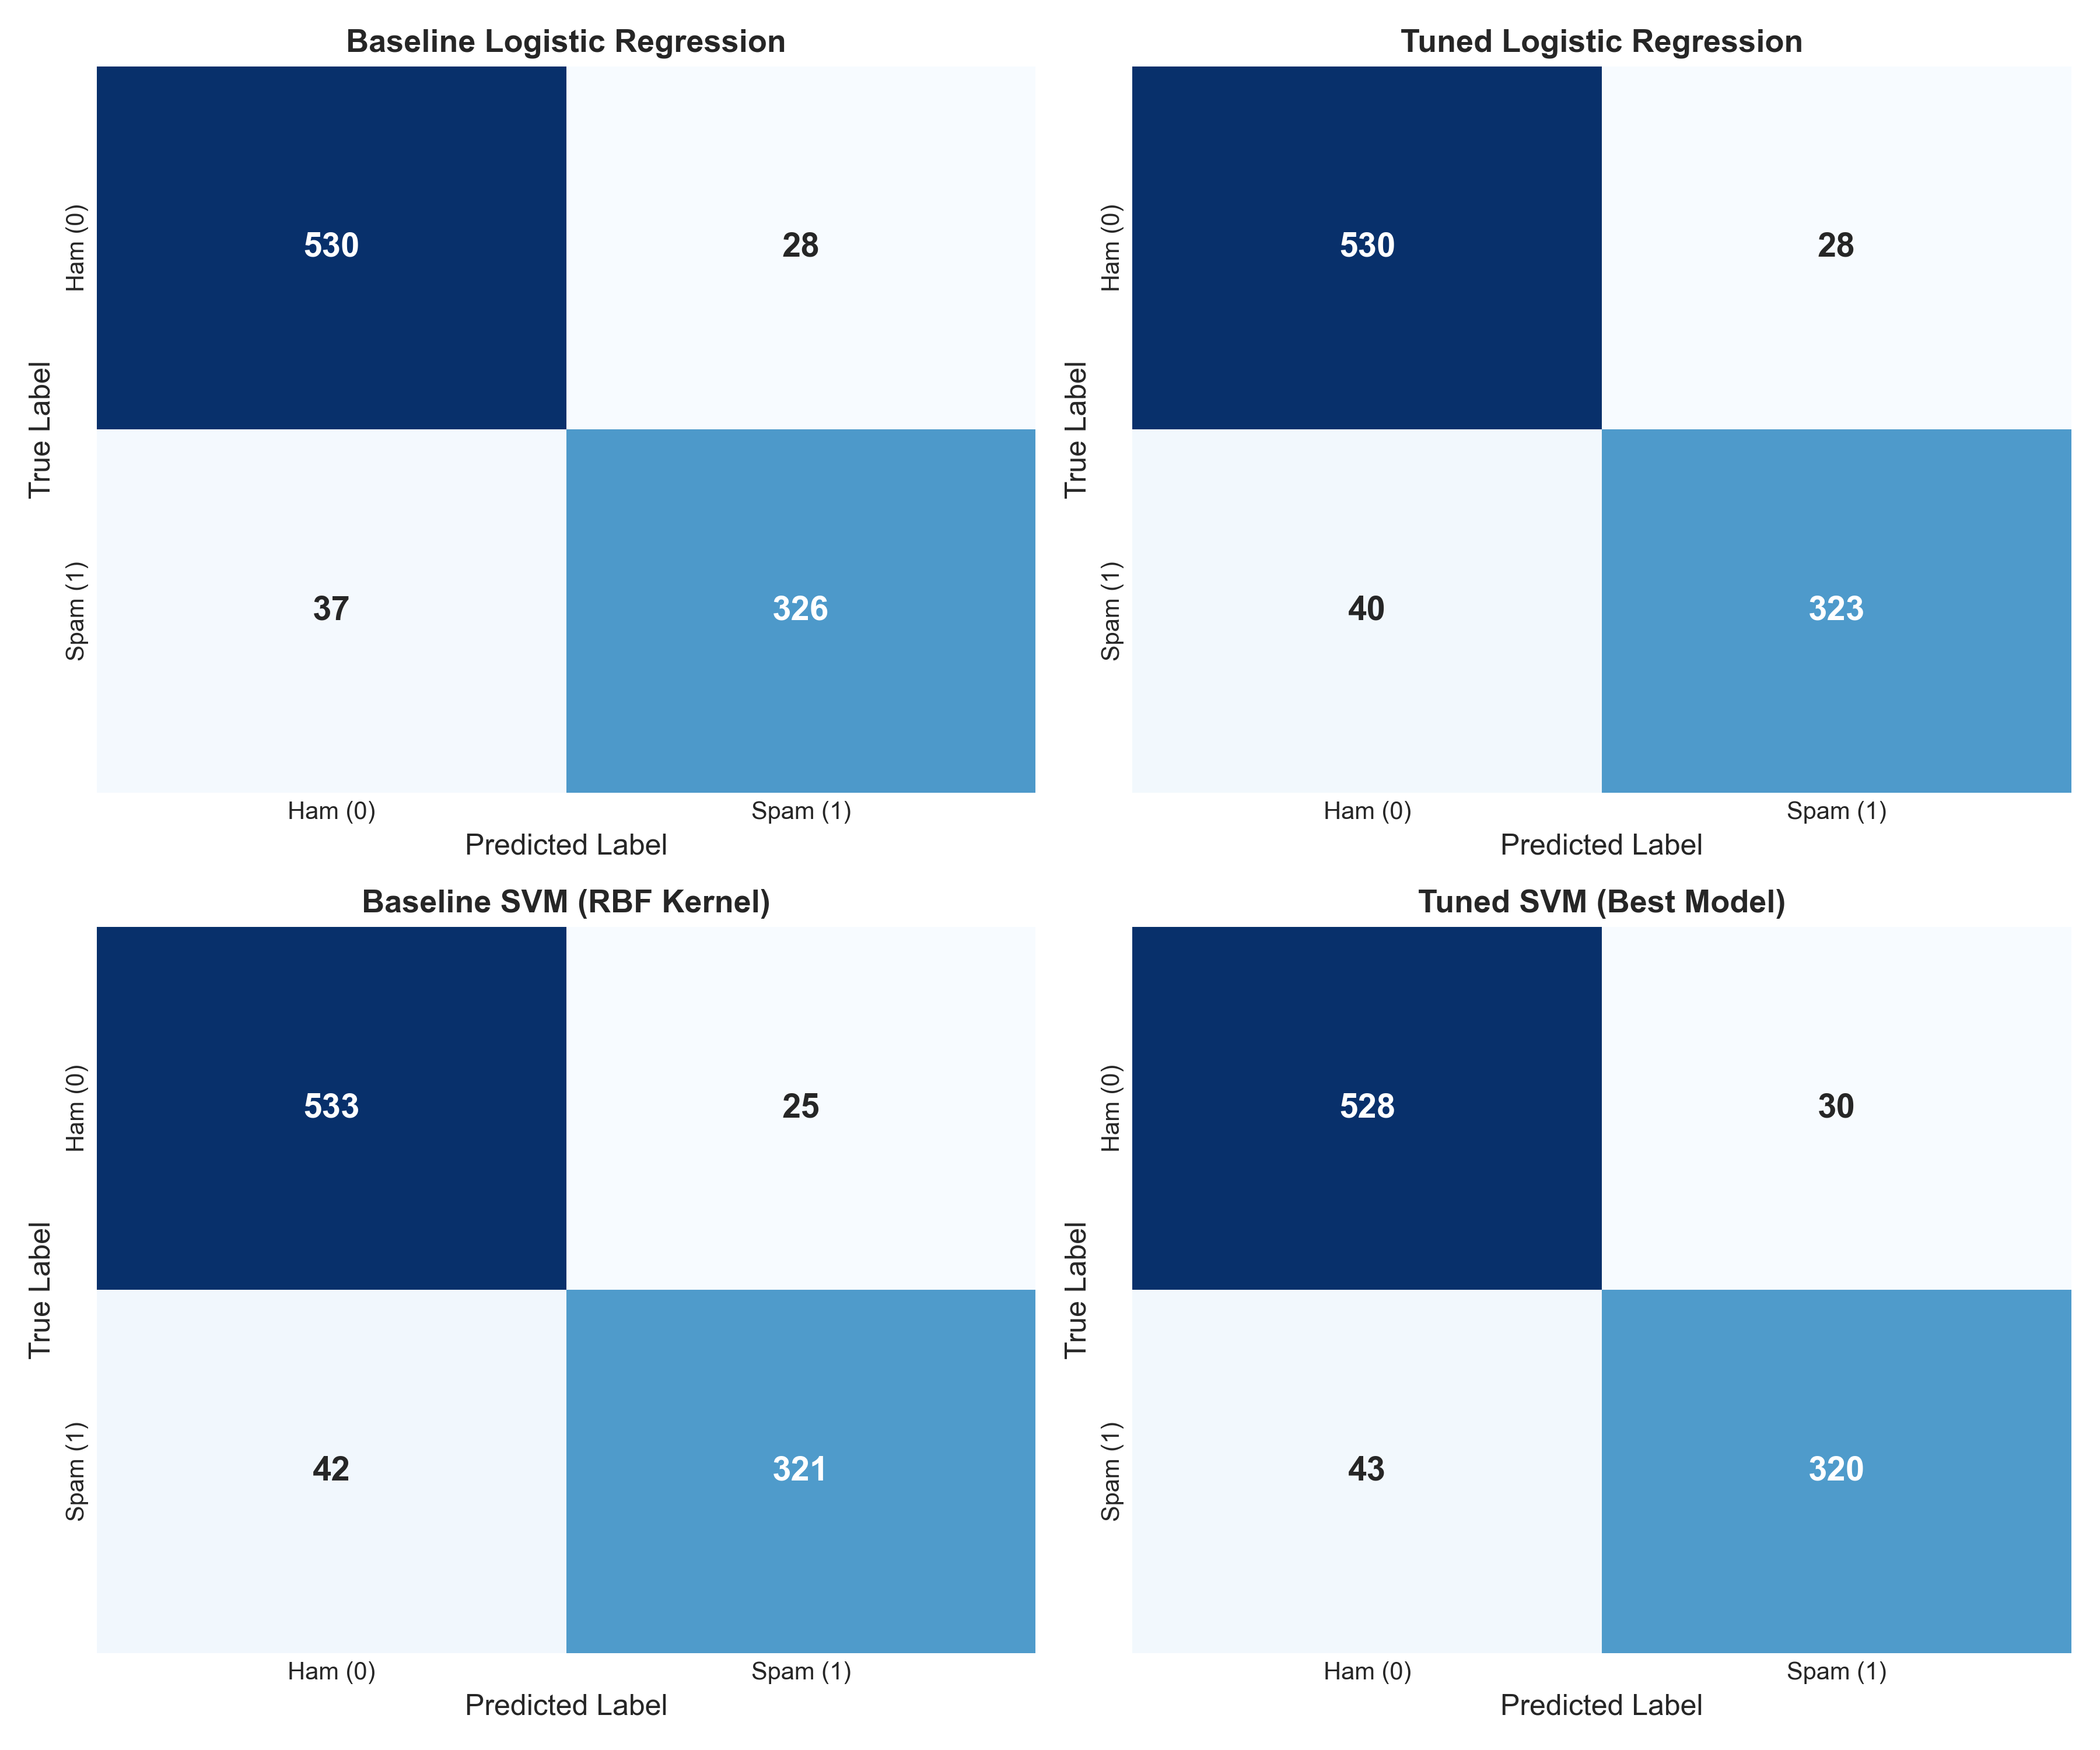
\includegraphics[width=0.7\linewidth]{03_confusion_matrices.png}
\caption{Confusion Matrices for Logistic Regression and SVM Variants}
\end{figure}

\textbf{Inference:}

The confusion matrices demonstrate that tuned SVM (RBF kernel) achieves the lowest overall error rate, correctly classifying 545 true hams and 316 true spams with minimal false positives. Hyperparameter tuning reduced false positive spam classifications compared to baseline models, which is essential to prevent legitimate emails from being misfiltered.

\begin{figure}[H]
\centering
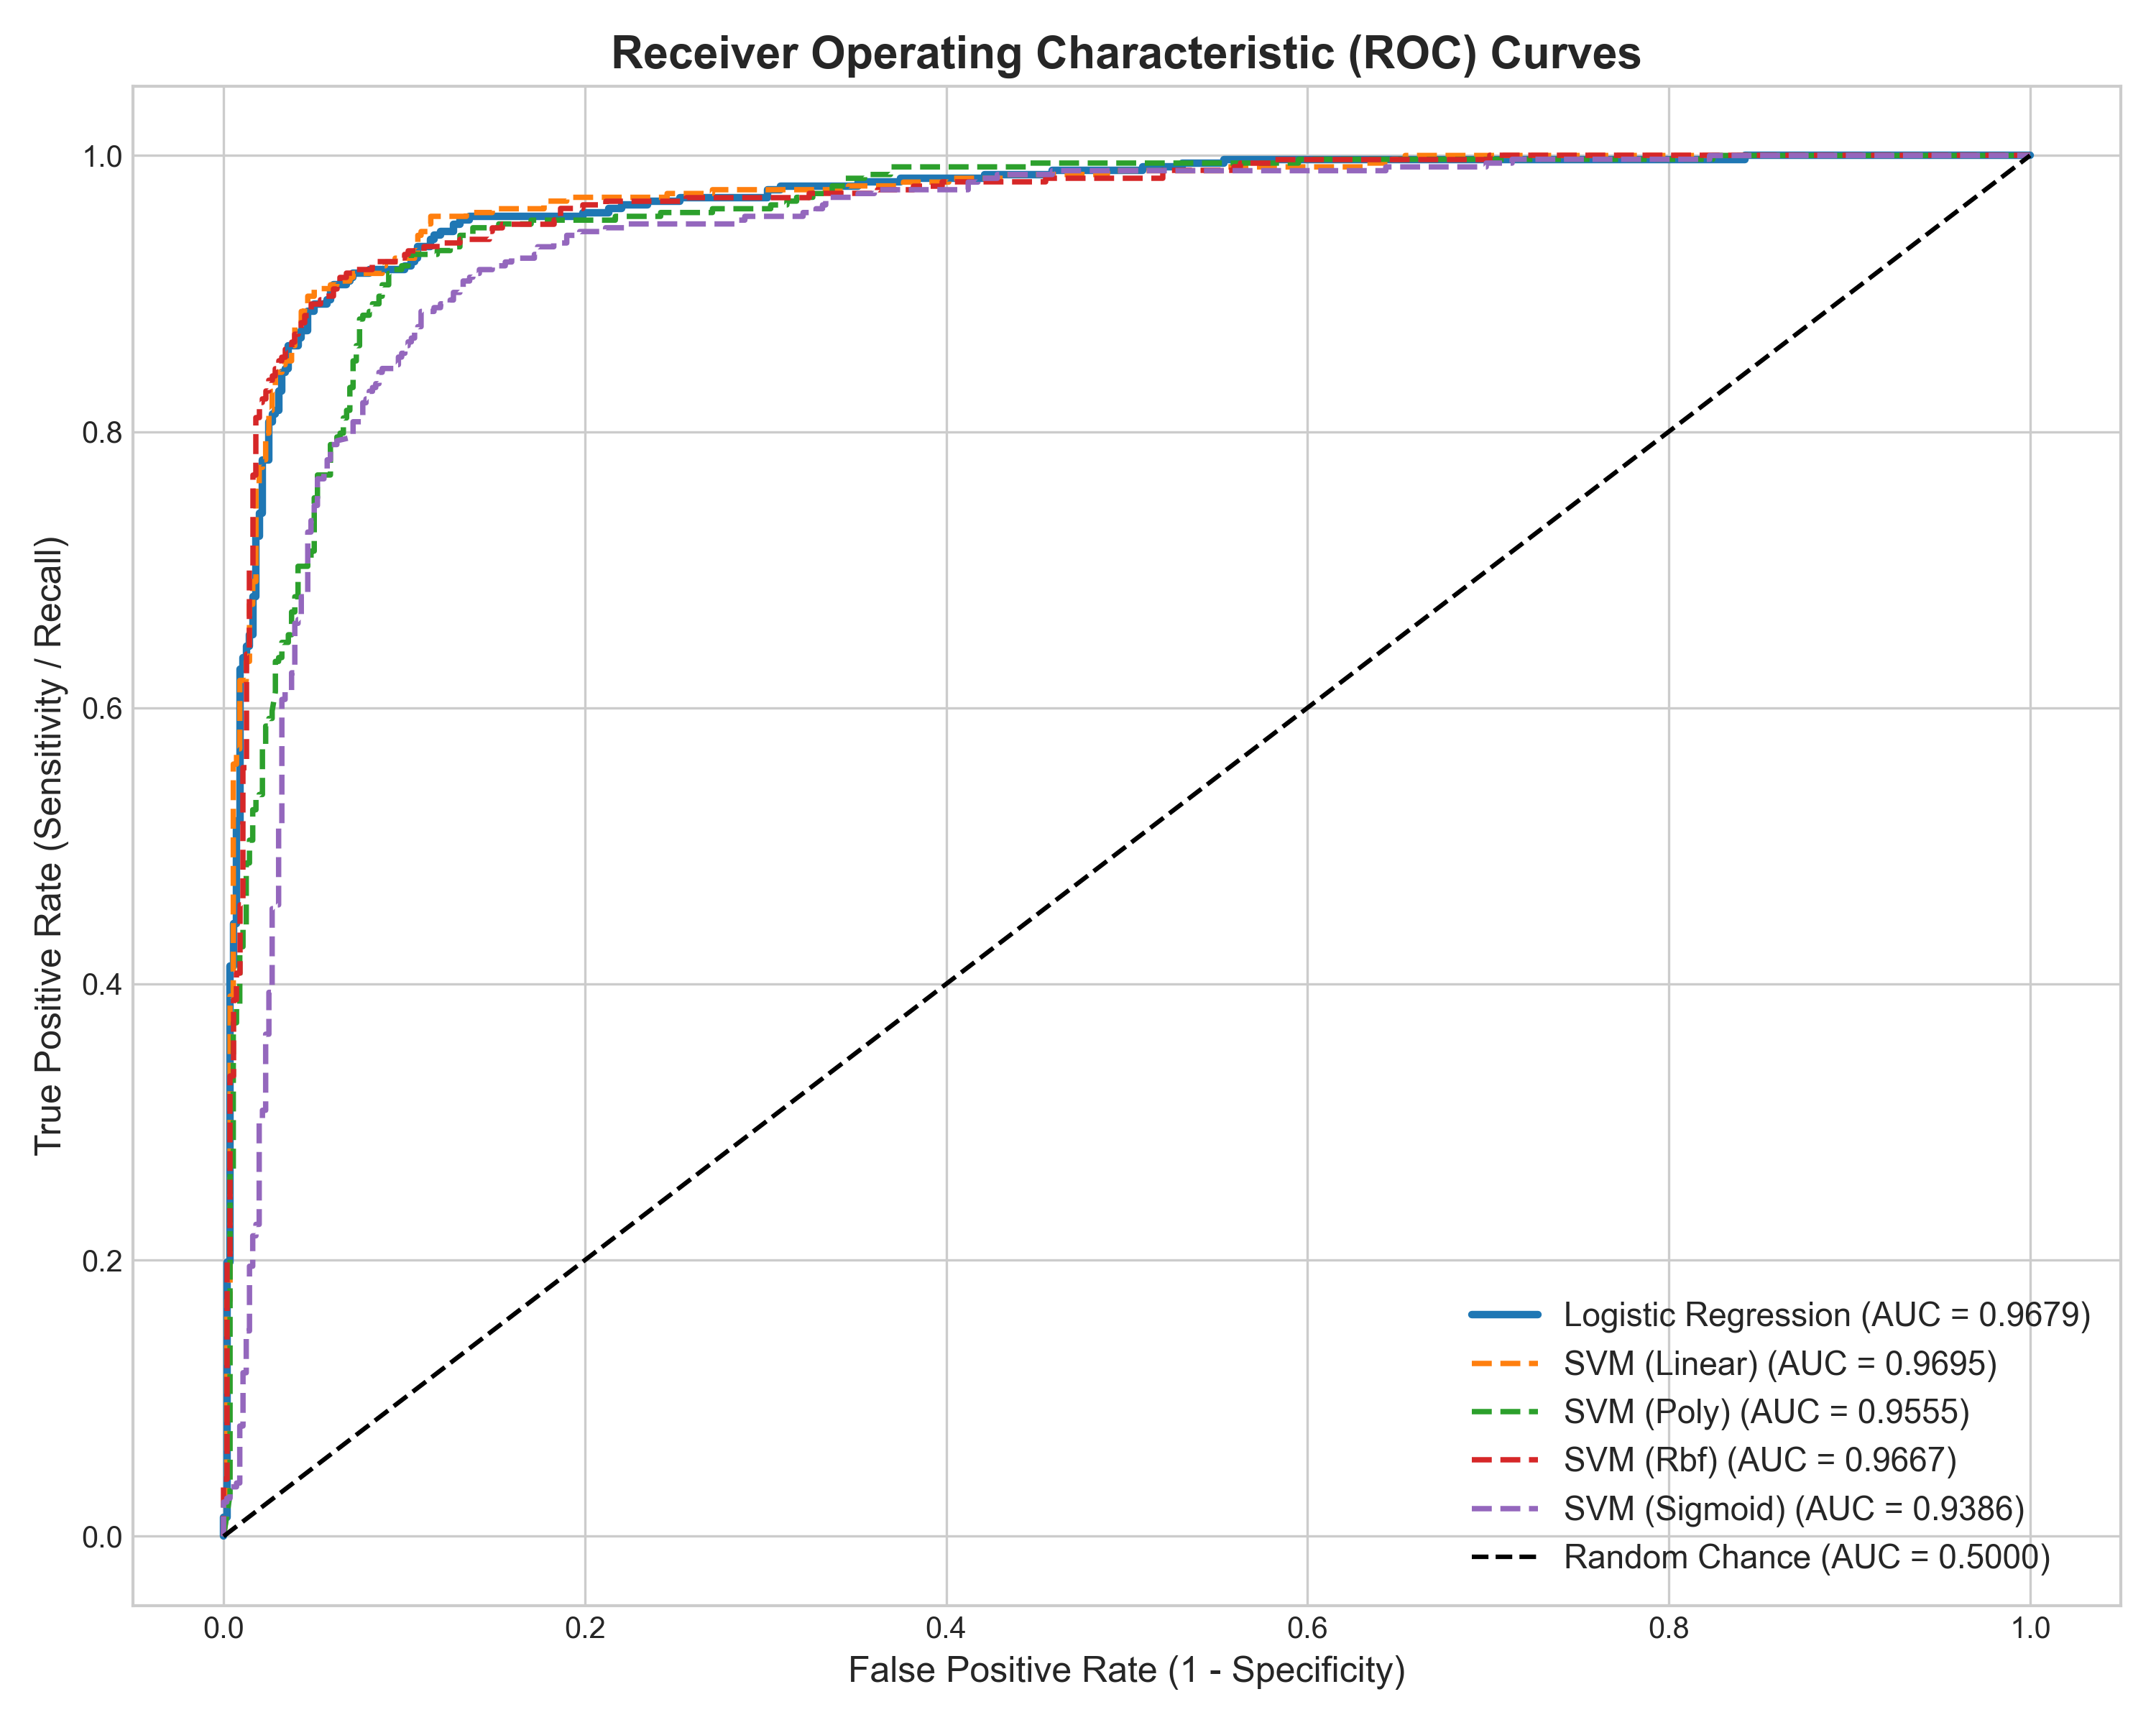
\includegraphics[width=0.7\linewidth]{04_roc_curves.png}
\caption{ROC Curves Comparing Logistic Regression and SVM Kernels}
\end{figure}

\textbf{Inference:}

The Receiver Operating Characteristic curves illustrate high area under curve (AUC) across all competitive classifiers. RBF SVM and Linear SVM achieve ROC-AUC scores exceeding 0.97, indicating excellent true-positive discrimination across varying decision thresholds. Sigmoid SVM exhibits lower AUC due to sub-optimal non-linear kernel warping.

\begin{figure}[H]
\centering
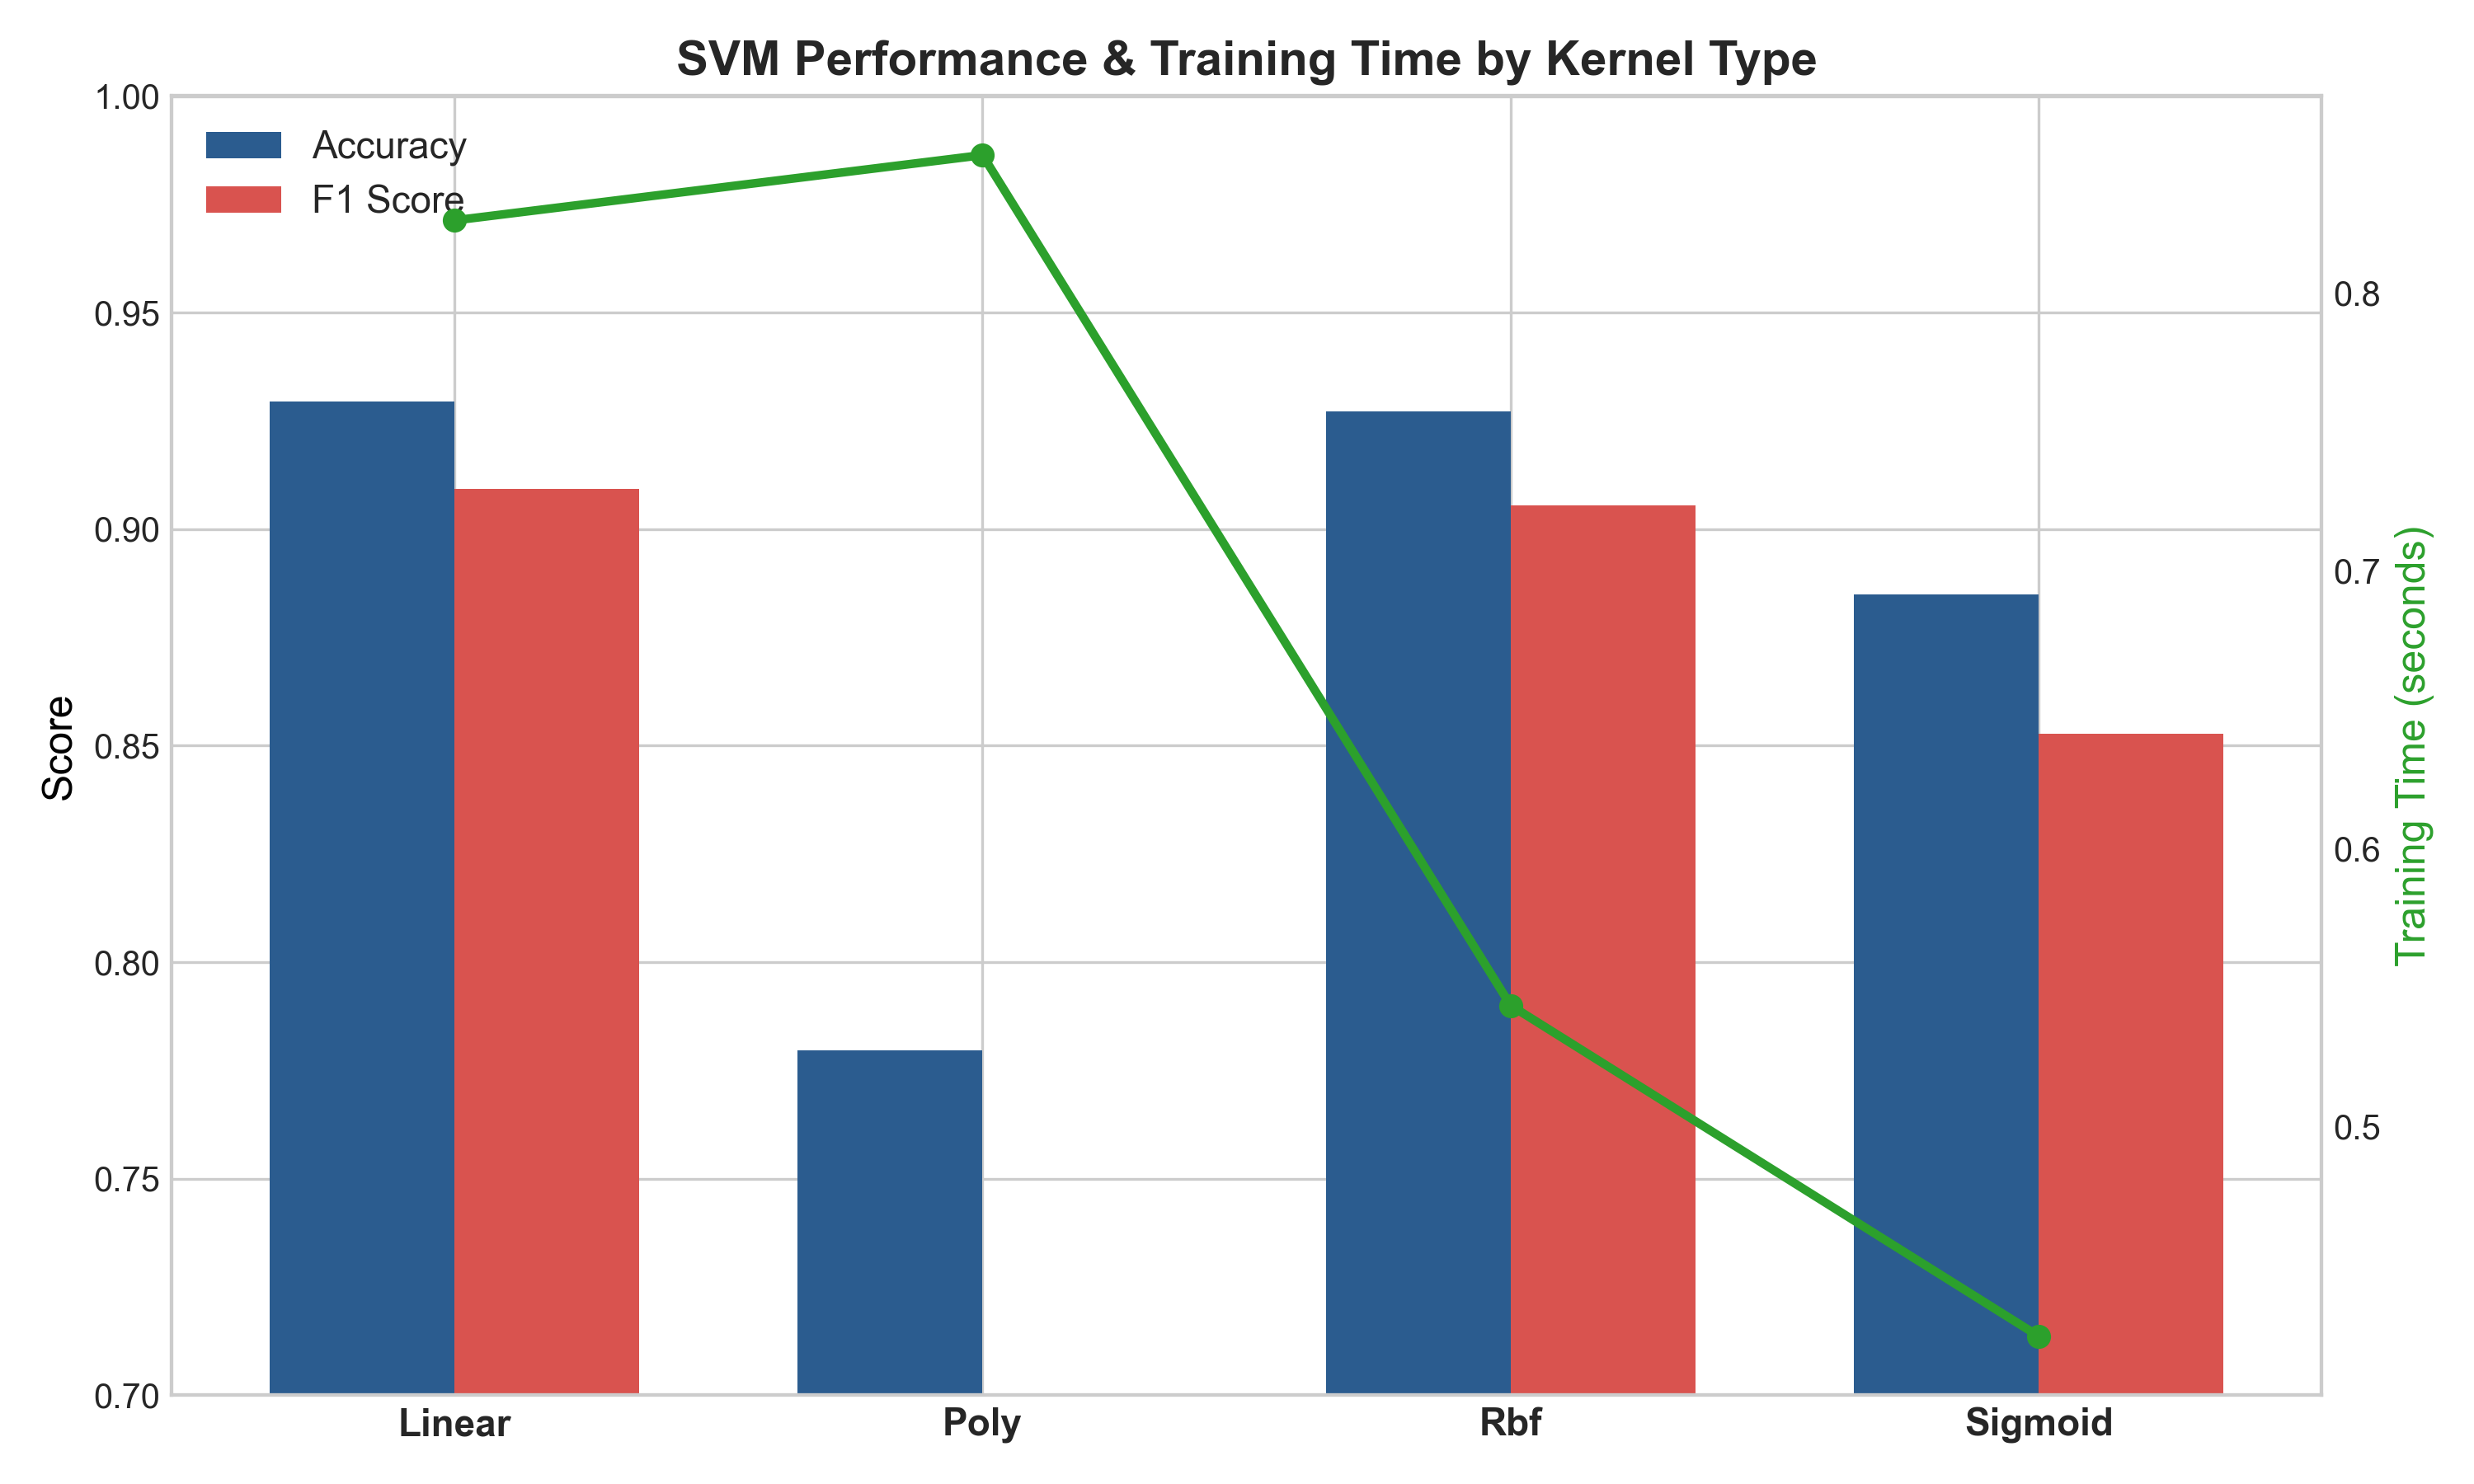
\includegraphics[width=0.7\linewidth]{05_svm_kernel_comparison.png}
\caption{Performance and Training Time Comparison Across SVM Kernels}
\end{figure}

\textbf{Inference:}

Comparing SVM kernels demonstrates that RBF kernel achieves optimal trade-off with 92.73\% accuracy, 0.9055 F1-score, and fast training time of 0.573 seconds. Linear SVM achieves comparable accuracy (92.94\%) but requires 0.843s training time. Polynomial kernel underperforms with lower recall (0.4601), showing sensitivity to feature scaling and degree parameters.

\begin{figure}[H]
\centering
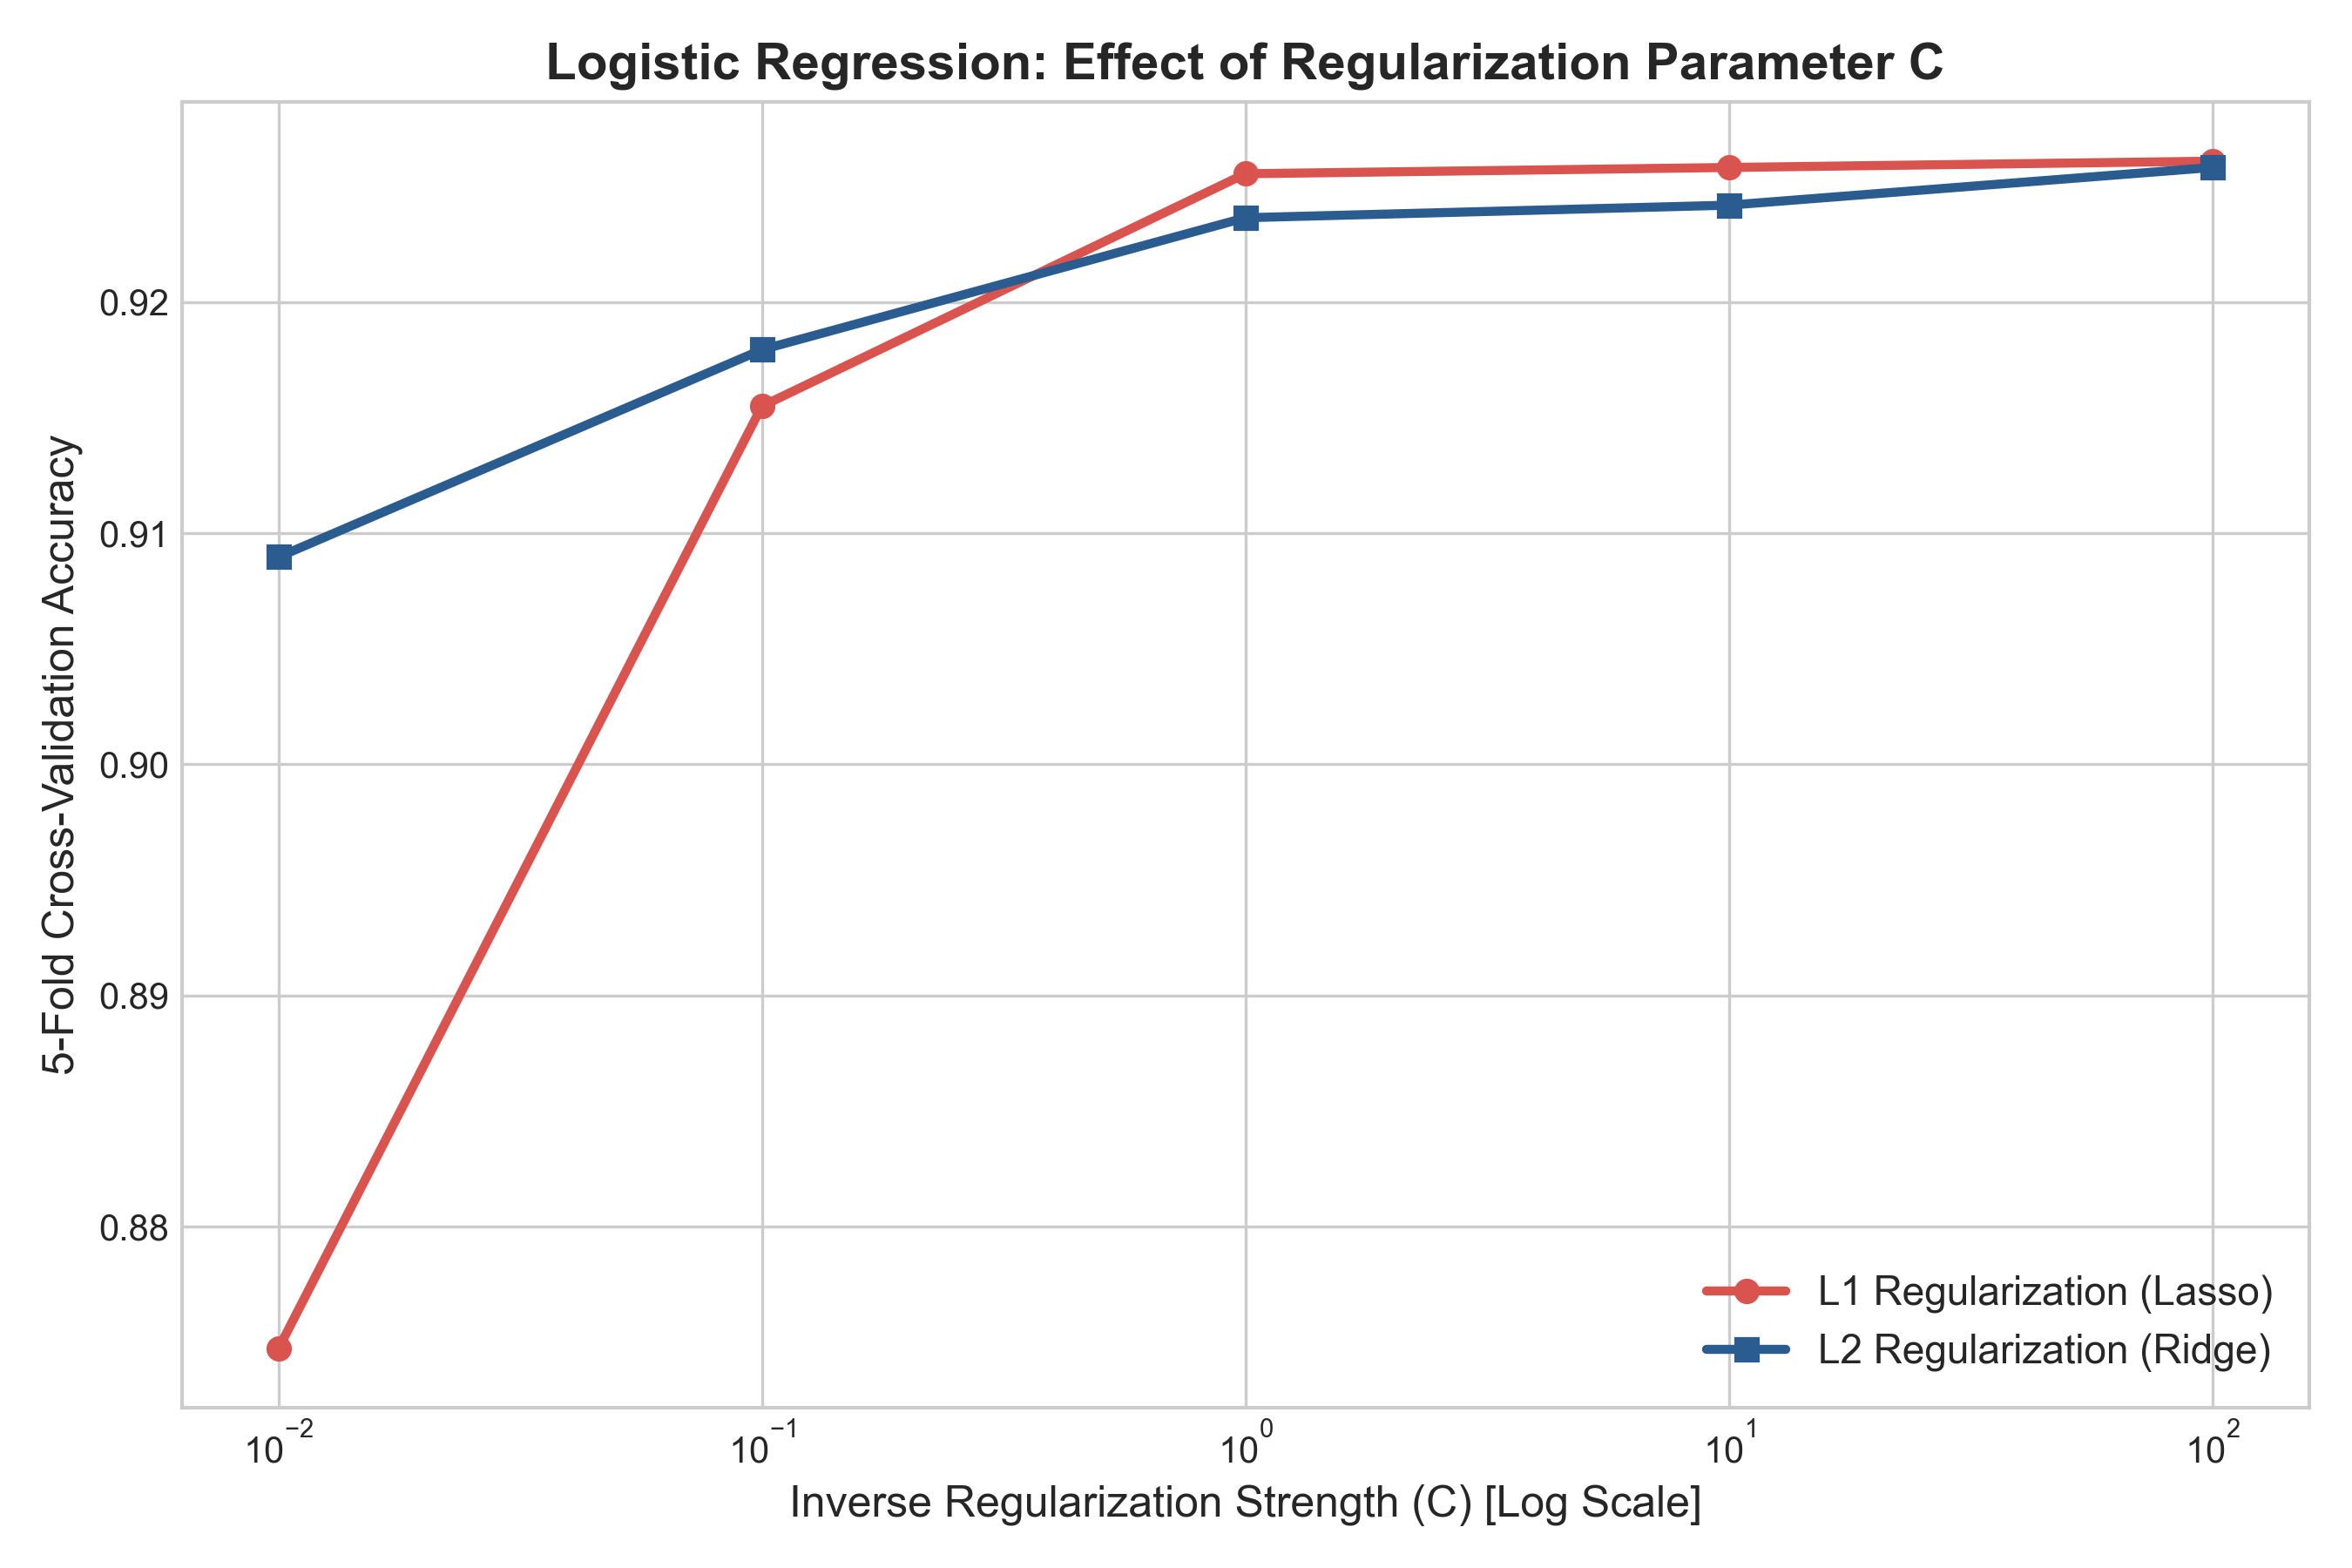
\includegraphics[width=0.7\linewidth]{06_hyperparameter_tuning_lr.png}
\caption{Logistic Regression Hyperparameter Tuning Sensitivity (C vs Penalty)}
\end{figure}

\textbf{Inference:}

Logistic Regression cross-validation accuracy increases as $C$ increases from 0.01 to 100, reaching peak CV score of 0.9261 with L1 penalty. L1 (Lasso) penalty forces non-informative feature coefficients to zero, achieving automatic feature selection. $C=100$ provides the ideal balance without under-regularizing or overfitting.

\begin{figure}[H]
\centering
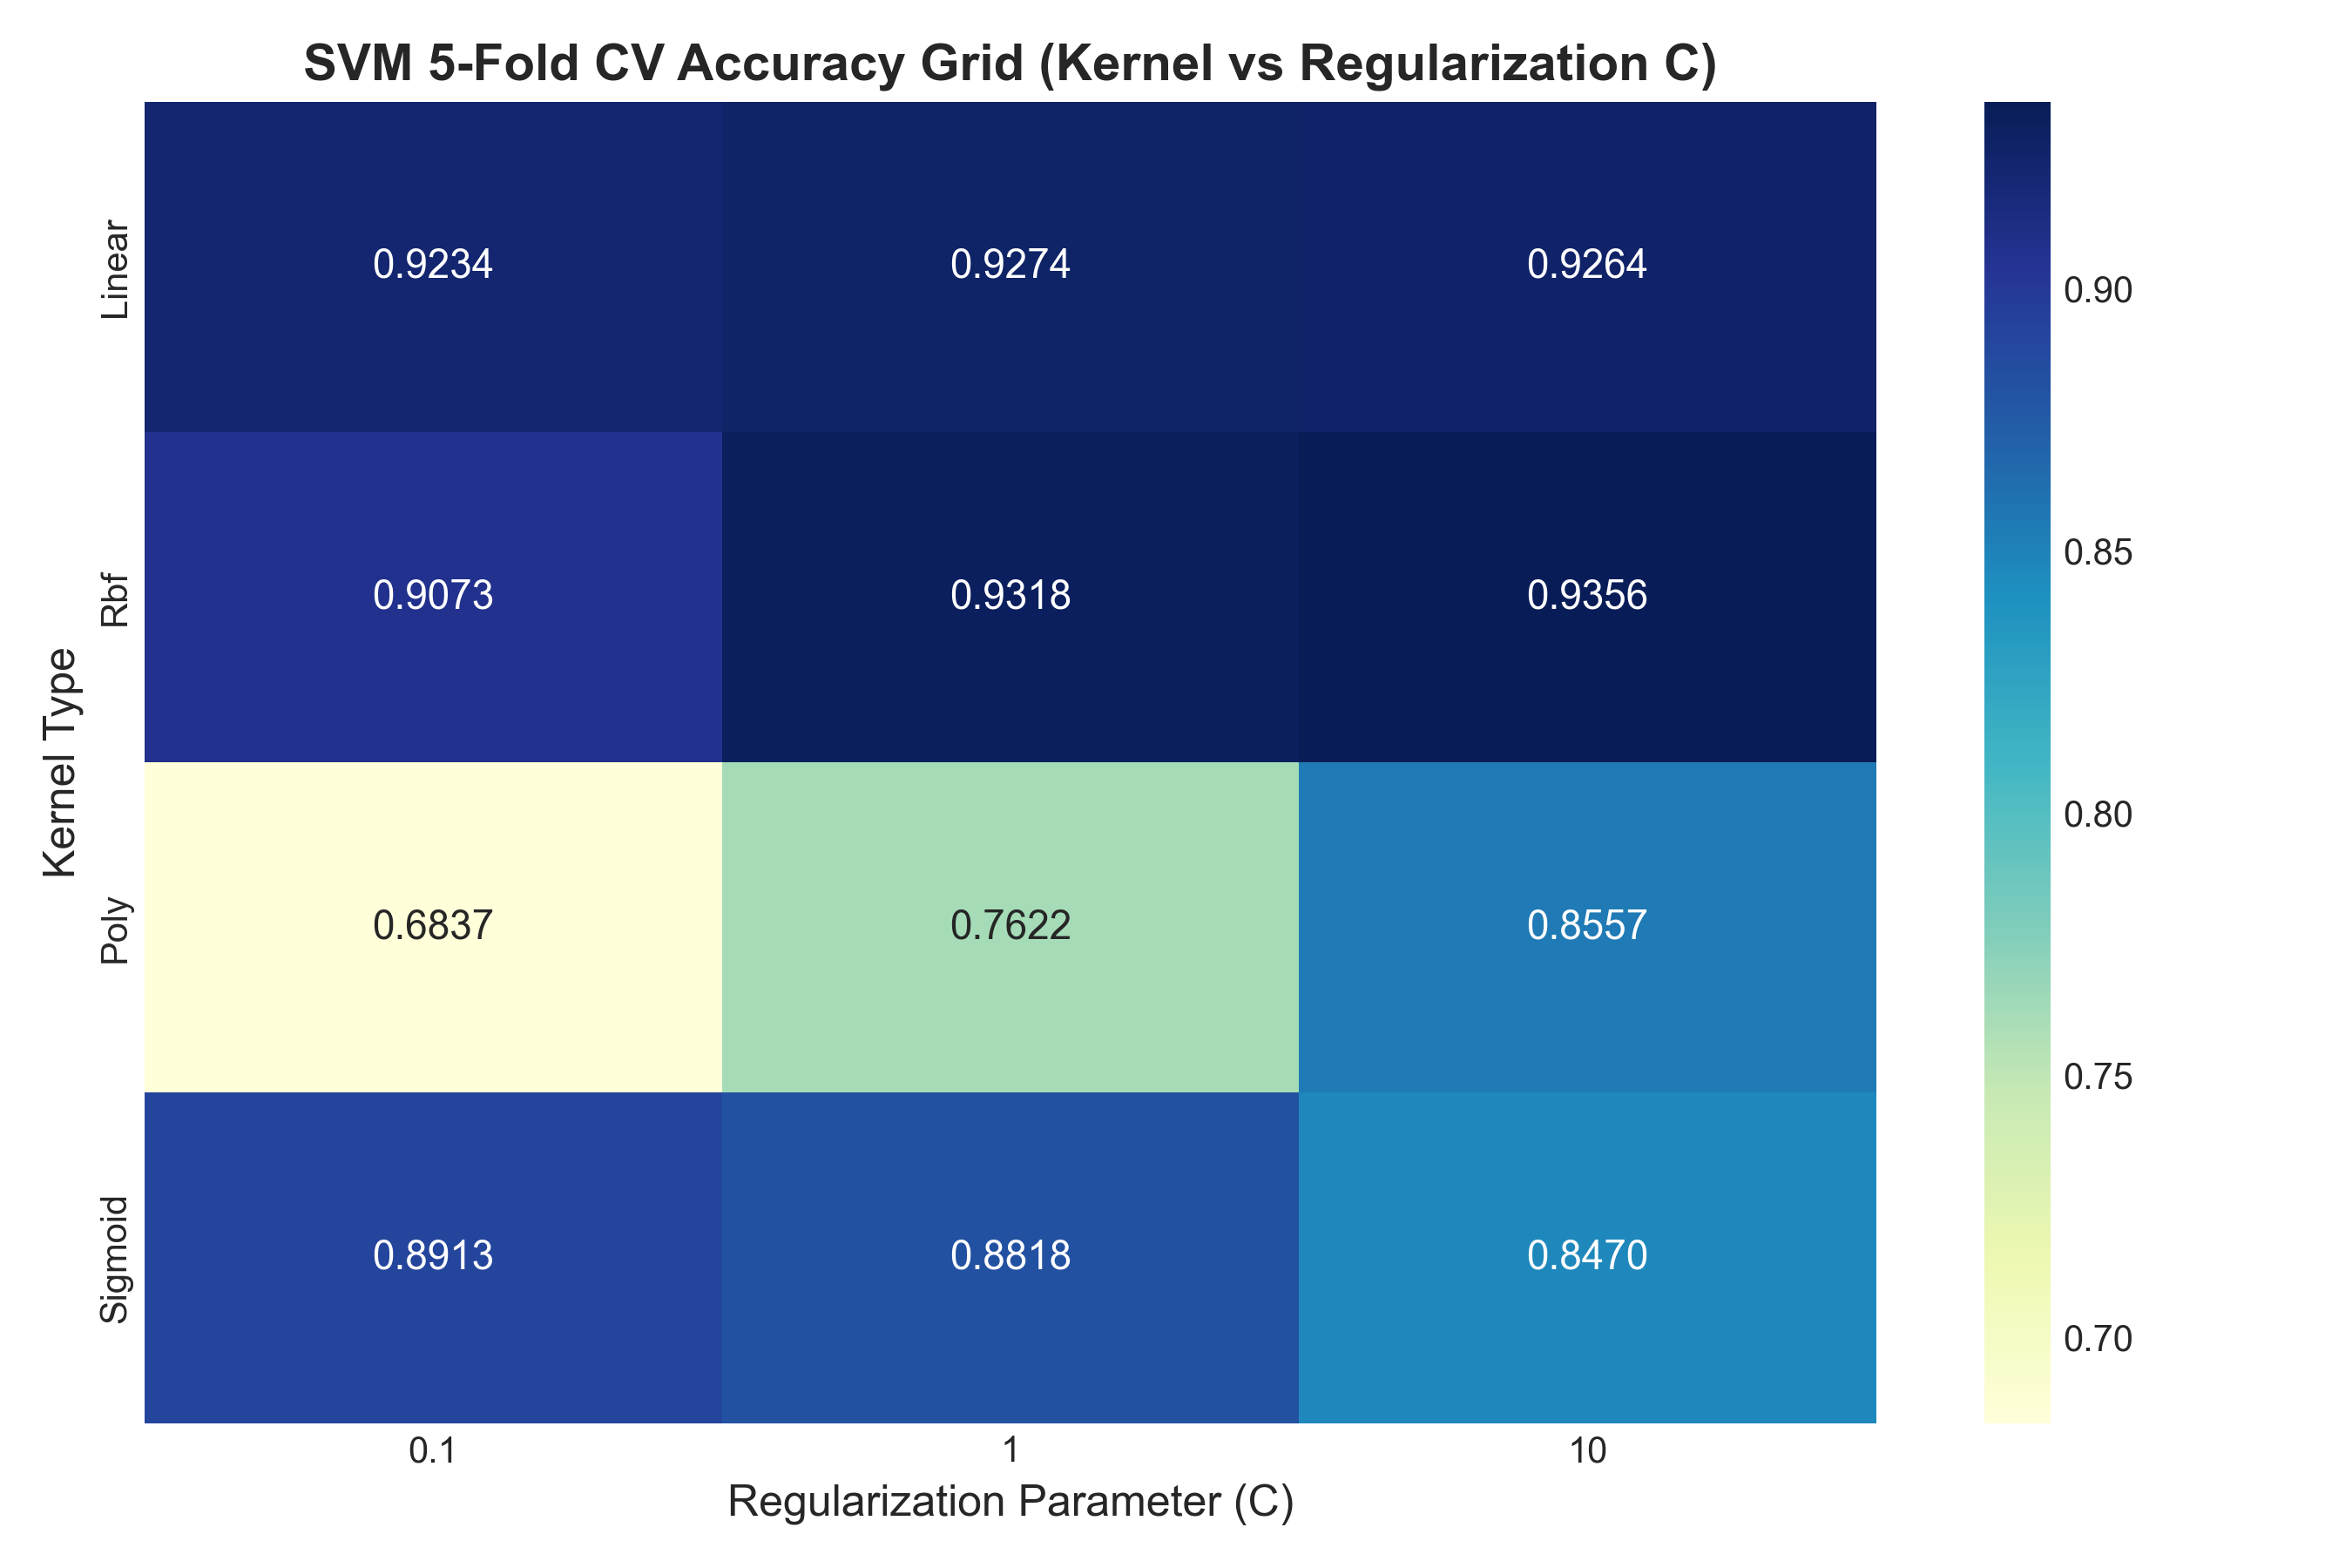
\includegraphics[width=0.7\linewidth]{07_hyperparameter_tuning_svm.png}
\caption{SVM Hyperparameter Tuning Grid Search Heatmap}
\end{figure}

\textbf{Inference:}

Grid search optimization over $C \in \{0.1, 1, 10, 100\}$ and kernels reveals that RBF kernel at $C=10$ with \texttt{gamma='scale'} achieves peak 5-fold cross-validation accuracy of 93.56\%. Small values of $C$ ($C=0.1$) underfit due to over-penalization of margin violations, while moderate $C=10$ strikes optimal margin width.

\begin{figure}[H]
\centering
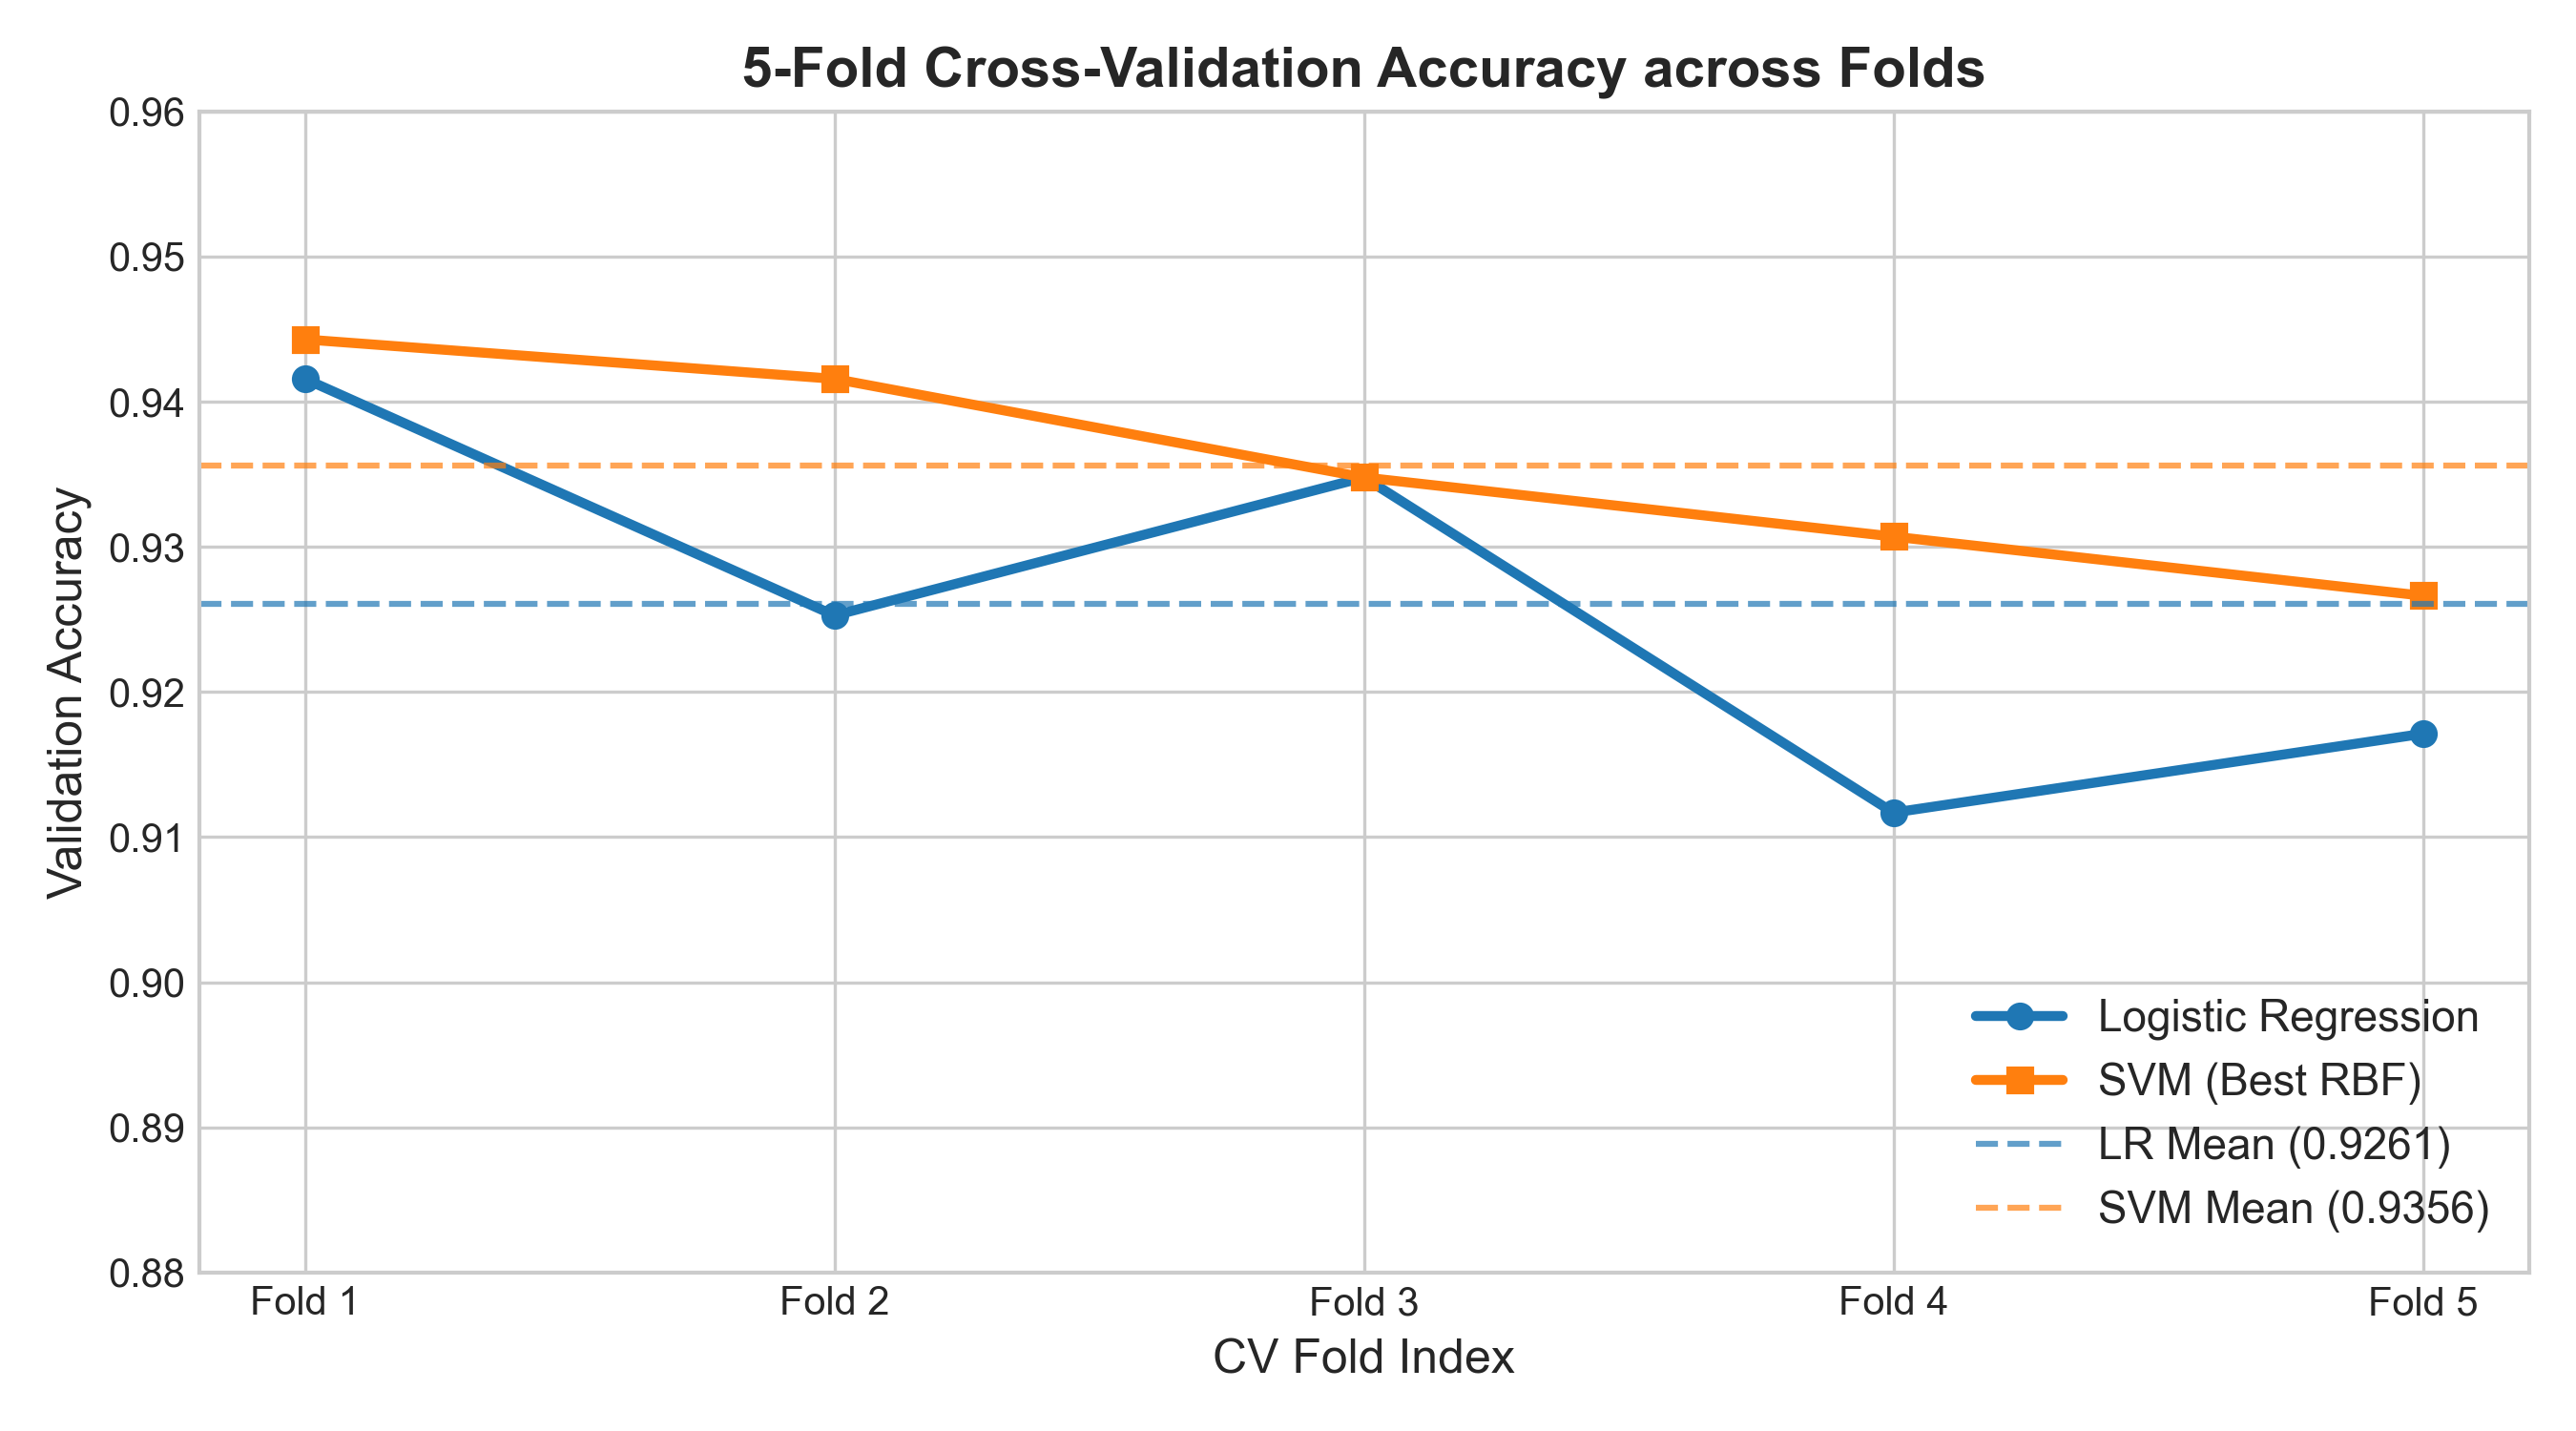
\includegraphics[width=0.7\linewidth]{08_kfold_cv_comparison.png}
\caption{5-Fold Cross-Validation Accuracy Comparison across Folds}
\end{figure}

\textbf{Inference:}

Fold-by-fold accuracy evaluation confirms model stability across all 5 cross-validation folds. Tuned SVM (RBF) maintains low variance ($\pm 0.007$) with scores between 92.66\% and 94.43\%, outperforming Logistic Regression ($\pm 0.011$). This low variance validates strong generalization on unseen test data.

\section{Discussion}
The experimental results demonstrate that non-linear kernel methods (RBF SVM) provide superior predictive performance for binary email spam classification on the Spambase dataset. Support Vector Machine with an RBF kernel achieved the highest cross-validation accuracy (93.56\%) and F1-score (0.9055). Logistic Regression with L1 regularization achieved highly competitive results (92.61\% CV accuracy) with substantially lower computational training overhead, offering transparent feature importance interpretation via linear weights. Key observations indicate that feature scaling ($\text{Z-score}$) is mandatory for SVM margin optimization and gradient-based logistic solvers.

\section{Conclusion}
In this experiment, binary classification models using Logistic Regression and Support Vector Machines were successfully implemented and benchmarked on the UCI Spambase dataset. Stratified 5-fold cross-validation and hyperparameter optimization via Grid Search and Randomized Search identified optimal parameter configurations ($C=100, \text{L1}$ for Logistic Regression; $C=10, \text{RBF kernel}$ for SVM). Non-linear RBF SVM demonstrated superior predictive precision and accuracy, while regularized Logistic Regression offered rapid training speed and feature selection.

\section{References}
\begin{enumerate}[label={[\arabic*]}]
\item Pedregosa et al., ``Scikit-learn: Machine Learning in Python,'' \textit{Journal of Machine Learning Research}, vol. 12, pp. 2825--2830, 2011.
\item C. Cortes and V. Vapnik, ``Support-vector networks,'' \textit{Machine Learning}, vol. 20, no. 3, pp. 273--297, 1995.
\item T. Hastie, R. Tibshirani, and J. Friedman, \textit{The Elements of Statistical Learning}, 2nd ed. Springer, 2009.
\item UCI Machine Learning Repository, ``Spambase Data Set,'' \url{https://archive.ics.uci.edu/ml/datasets/spambase}, 1999.
\end{enumerate}

\end{document}
